\chapter{光分析导论}
\begin{introduction}[重点]
    \item Beer-Lambert定律
    \item 数据处理方法
    \item 光学系统
\end{introduction}
\begin{introduction}[难点]
    \item 标准曲线法
    \item 标准加入法
    \item 内标法

\end{introduction}
\section{电磁辐射与物质的相互作用}
从对彩虹的观察中我们知道,可见光(白光)由从紫色到红色的连续颜色组成。如果一束
白光通过水烧杯,保持白色。如果将高锰酸钾添加到水中,白光穿过溶液后会变成紫色。
高锰酸盐溶液允许白光的红色和蓝色成分通过,但会吸收原始光束中的其他颜色。
这是\emph{电磁辐射}或光与物质相互作用的一个例子。在这种情况下,电磁辐射是可见光
,我们可以用眼睛看到吸收某些光的效果。但是,电磁辐射与物质之间的相互作用以多种
方式发生,并且辐射能范围很广。这些相互作用中的大多数不是人眼可见的,而是可以
用合适的仪器测量的。

电磁辐射与物质的相互作用不是偶然的,而是关于吸收或发射的光的波长,以及吸收或
吸收的程度遵循有据可查的规则。光谱学的主题是电磁辐射与物质相互作用的研究。

\subsection{电磁辐射}
多年以来,电磁辐射的性质使科学家感到困惑。有时,光看起来像波;在其他时候,它的
行为好像是由小颗粒组成的。尽管我们现在已经了解包括电磁辐射在内的所有物质的
“波粒二象性”,但从量子力学的角度来看,在许多情况下将电磁辐射视为具有波的属性
仍然很方便。可以表示光波为振荡垂直的电场和磁场。场彼此成直角,并且与光的传播
方向成直角。
\begin{figure}[htbp]
    \centering
    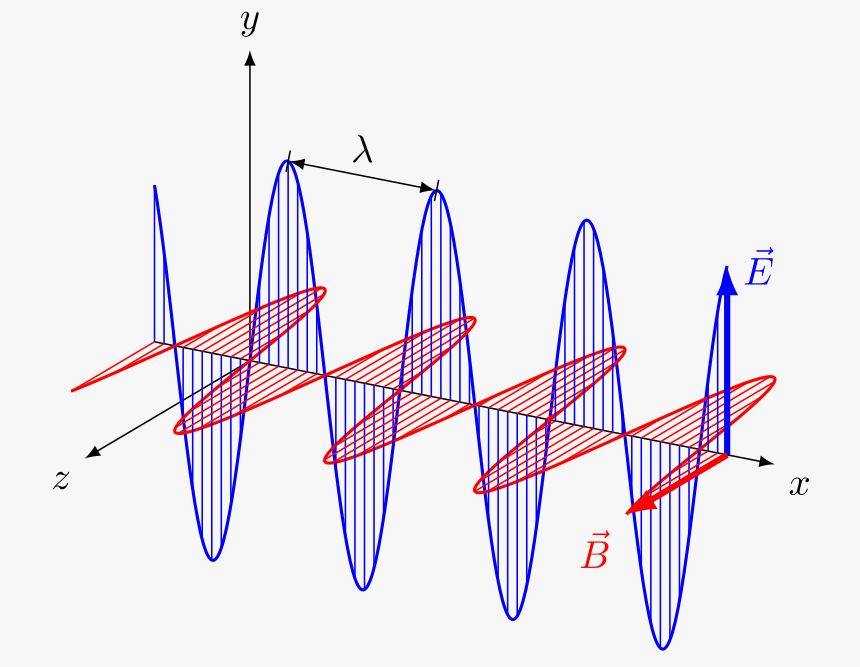
\includegraphics[width=0.85\textwidth]{ElectromagneticWavesPropagation.png}
    \caption{光沿着$x$方向传播,$y$方向为电场,$z$方向为磁场,$\lambda$为波长}
    \label{fig:EMwave}
\end{figure}

如图\ref{fig:EMwave}所示,振荡为正弦曲线。我们可以轻松、准确地测量波长$\lambda$
,定义为两个
连续最大值之间的波峰到波峰的距离。波长的标准单位是长度的SI单位,米($m$),
但是通常使用较小的单位,例如厘米($cm$),微米($\mu m$)和纳米($nm$)。波的
振幅定义为从原点到振荡的点位移的矢量的最大值。仅沿一个轴传播的光波
电场部分的示例如图\ref{fig:EMwave}所示。仅限于一个平面的这种波称为平面偏振光。
所示的波仅代表单个波长$\lambda$。仅一种波长的光称为单色光。包含多个波长的光
称为多色光。白光是多色光的一个示例。波的频率$\nu$是每秒通过固定点的波峰数。
波的波峰间振荡称为周期。频率的通用单位是赫兹($Hz$)或倒数秒($s^{-1}$);
频率的较旧术语是每秒的周期数($cps$)。一赫兹等于每秒一个周期。
光的波长$\lambda$和频率$\nu$满足下式
\begin{equation}
    c = \lambda\nu
    \label{eq:1st}
\end{equation}
其中,$c$为真空中光速,$2.997\times 10^8 m/s$;$\nu$频率,单位为$Hz$;$\lambda$
波长,单位为$m$。

真空中,光速最大,且与波长无关。频率由光源决定,并且不会变化。当光通过非真空的
材质,其速度会降低。因为频率不能改变,波长减小。空气中的光速,它与
真空中的光速相差很小。通常,我们将$3.00\times 10^8 m/s$(三位有效数字)用于空气
或真空中的光速。在某些情况下,将光视为粒子流会更方便。光的粒子成为光子。光子的
特征在于能量$E$与频率有关,关系式如下:
\begin{equation}
    E = h\nu
    \label{eq:2nd}
\end{equation}
其中,$E$为能量,单位是$J$,$h$是普朗克常数,$6.626\times 10^{-34} Js$,$\nu$
是频率,单位是$Hz$。联立式(\ref{eq:1st})和(\ref{eq:2nd}),可得
\begin{equation}
    E = \frac{hc}{\lambda}
    \label{eq:3th}
\end{equation}
\begin{figure}[htbp]
    \centering
    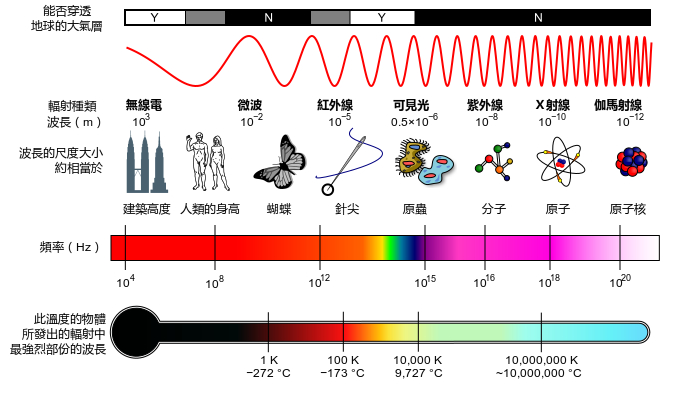
\includegraphics[width=0.85\textwidth]{wave.jpg}
    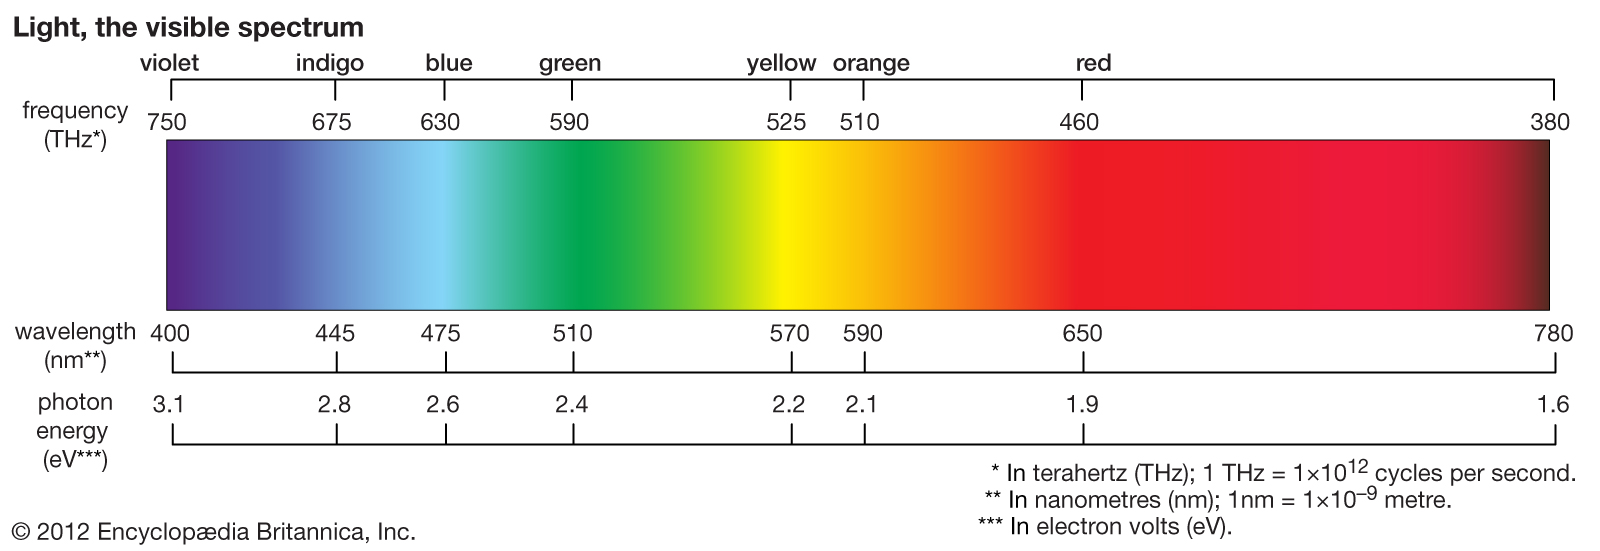
\includegraphics[width=0.85\textwidth]{visual.jpg}
    \caption{电磁波谱}
    \label{fig:wavegraph}
\end{figure}
从式(\ref{eq:2nd})和(\ref{eq:3th})的关系可以看出,电磁辐射的能量与频率成正比,
与波长成反比。电磁辐射的范围从极低能量(长波,低频)的辐射(如无线电波和微波)
到极高能量(短波,高频)的辐射(如X射线)。作为分析化学家,我们感兴趣的电磁谱
的主要区域如图(\ref{fig:wavegraph})所示。从该图清楚可见,可见光,即人眼所响应
的电磁频谱的一部分,仅占所有辐射能的很小一部分。表(\ref{tab:1st})列出了各种类
型电磁辐射的一些常用单位和符号。
\begin{table}[htbp]
    \centering
    \caption{电磁辐射波长符号和单位}
    \label{tab:1st}
    \begin{tabular}{lccl}
        \hline
        {\bf Unit}&{\bf Symbol}&{\bf Length ($m$)}&{\bf Type of Radiation}\\
        \hline
        Angstrom & \AA& $10^{-10}$&x-ray\\
        Nanometer& $nm$& $10^{-9}$&UV/Vis\\
        Micrometer& $\mu m$& $10^{-6}$&Infrared (IR)\\
        Millimeter& $mm$& $10^{-3}$&IR\\
        Centimeter& $cm$& $10^{-2}$&Microwave\\
        Meter& $m$& $1$&Radio\\
        \hline
    \end{tabular}
\end{table}
\subsection{电磁辐射与物质的相互作用}
光谱学是研究辐射能(光)与物质相互作用的方法。从量子力学中我们知道,能量实际上
只是物质的一种形式,所有物质都具有波和粒子的特性。但是,由以固体,液体或气体
形式存在的分子,原子或离子组成的物质主要表现出粒子的特性。光谱学研究光与物质的
相互作用,物质定义为由分子或原子或离子组成的材料。

在气体中,原子或分子彼此广泛分离;在液体和固体中,原子或分子紧密相连。在固体中
,原子或分子可以像许多矿物中那样排列成高度有序的阵列(称为晶体),也可以像许多
塑料中一样无规排列或无定形。无论原子,分子和离子的物理状态或排列如何,它们都在
不断运动。对于分子,涉及许多类型的运动。分子可以转动,振动和平移(在空间中到处
移动)。与辐射能的相互作用会影响这些分子运动。吸收红外辐射的分子振动幅度更大;
与UV/VIS光的相互作用可将键合电子移动到分子中更高的能级。任何形式的运动或电子能
级的变化都涉及分子能量的变化。能量的这种变化称为\emph{跃迁}。分子有可能发生
振动跃迁,转动跃迁和电子跃迁。原子和离子也有一些相同类型的运动。原子可以在
空间中移动,其电子可以在能级之间移动,但是原子和单原子离子不能转动或振动。
物质的化学性质(其组成),其物理状态以及处于物理状态的原子或分子彼此之间的
排列会影响任何给定材料与电磁辐射相互作用的方式。表\ref{tab:2nd}列出了通过光谱
学研究的一些重要的跃迁类型。我们将在后面的章节中详细介绍这些技术。实际上,有数
百种用于研究物质的跃迁类型和光谱学类型,我们介绍最常见的分析光谱类型。

\begin{table}[htbp]
    \centering
    \caption{光谱研究的几种典型转换}
    \label{tab:2nd}
    \begin{tabular}{lll}
        \hline
        转换类型& 光谱方法 & 波长范围 \\
        \hline
        磁场中核子自旋 & 核磁共振 & $0.5-10 m$\\
        分子转动与振动 & 拉曼和红外 & $0.8-300 \mu m$\\
        成键电子和价电子能级 & UV/VIS & $180-800 nm$\\
        核心电子能级 & X-ray & $0.1-100 $\AA\\
        \hline
    \end{tabular}
\end{table}

当光照射到物质样品上时,光可能会被样品吸收,透射穿过样品,从样品表面反射或
被样品散射。样品在吸收入射光后也可以发光。这样的过程称为\emph{发光}。根据发生
的特定过程,有不同类型的发光,称为\emph{荧光}或\emph{磷光}。发光也可能是由吸收
光以外的过程引起的。有基于所有这些相互作用的光谱方法。表\ref{tab:3th}总结了
光与物质相互作用的主要类型,并给出了基于这些相互作用的常见光谱技术的示例。
目前,我们将专注于物质对光的吸收、透射和发射。

\begin{table}[htbp]
    \centering
    \caption{几种光与物质的作用}
    \label{tab:3th}
    \begin{tabular}{lll}
        \hline
        相互作用 & 测量的辐射 & 光谱方法 \\
        \hline
        吸收(Absorption) &
        入射光(Incident light) $I_0$ & 原子吸收(Atomic absorption)\\
        传输(Transmission)&透射光(Transmitted light) $I$&分子吸收(Molecular absorption)\\
        \hline
        \multirow{3}*{\shortstack{吸收后发射\\(Absorption\\ then emission)}} & 
        \multirow{3}*{发射光(Emitted light) $I'$} & 原子荧光(Atomic fluorescence)\\
        &&分子荧光(Molecular fluorescence)\\
        &&分子磷光(Molecular phosphorescence)\\
        \hline
        \multirow{3}*{散射(Scattering)} &
        \multirow{3}*{散射光(Scattered light) $I_S$} &测浑法(Turbidimetry) \\ 
        &&浊度法(Nephelometry)\\
        &&拉曼(Raman)\\
        \hline
        \multirow{2}*{反射(Reflection)}&\multirow{2}*{反射光$I_R$}&全反射衰减
        (Attenuated total reflection)\\
        &&漫反射(Diffuse reflection)\\
        \hline
        \multirow{3}*{发射(Emission)}&\multirow{3}*{发射光(Emitted light)$I_e$}
        &原子发射(Atomic emission)\\
        &&分子发射(Molecular emission)\\
        &&化学发光(Chemiluminescence)\\
        \hline
    \end{tabular}
\end{table}

如果我们将白光(即可见光)穿过蓝色玻璃,则发出的光就是蓝色。玻璃吸收了其他颜色
,例如红色和黄色。我们可以通过蓝色玻璃发出红色光来确认这种吸收。如果吸收足够强
,则所有的红光都会被吸收;玻璃上没有光发出,而是黑色。如何解释呢?

电磁辐射与物质的相互作用符合量子力学定律。原子、离子和分子,以具有特定能量的某
些离散状态存在。依据量子力学定律,状态的改变需要吸收或发射能量$\Delta E$,该能
量等于始态和终态之间的能量差。能量状态是量子化的,状态变化(能量变化)可表示:
\begin{equation}
    \Delta E = E_{\text{final}} - E_{\text{initial}} = h\nu
    \label{diffEnergy}
\end{equation}
将$c = \lambda\nu$带入式(\ref{diffEnergy}),得
\begin{equation}
    \Delta E = h\nu=\frac{hc}{\lambda}
    \label{diffEnergy2}
\end{equation}
从式(\ref{diffEnergy2})可知,物质在两种状态跃迁时,吸收或发射辐射。物质仅仅能
吸收或发射特定频率(或波长)的辐射,对应于物质存在的两种状态的能量差。吸收辐射
$E_{\text{final}} > E_{\text{initial}}$,发射辐射$E_{\text{final}} <
E_{\text{initial}}$。$\Delta E$有正有负,在求解转换的波长和频率时,使用绝对值。
波长、频率和光速,总是正值。

特定的分子,如正己烷,或是特定的原子,如汞,能吸收或发射特定频率的辐射。所有正
己烷吸收和发射的频率是相同,这些频率不同于其它分子,例如苯。所有汞原子吸收相同
频率的入射光,这一频率与其它原子(如铅、铜)不同。不但频率是独特的,吸收或发射
的度也是独特的。给定强度的光的吸收或发射的度。化合物频率的独特性和每一个频率下
的吸收和发射的总量,是表征化合物的光谱学基础。我们称频率和强度为吸收或发射
光谱。

分子或原子最低能量状态称为基态。比基态高的,称为激发态。通常,室温下,分子和原子
都处于基态。

前例中蓝色玻璃能吸收红光和黄光,我们粗略的推测能量状态图。假设任何一种或几种光
穿过玻璃前,玻璃是基态,能量为$E_1$。玻璃吸收红光后,到达激发态,激发态与基态的
能量差为红光波长所具有的能量。从图\ref{fig:wavegraph}中,在可见光区域,选择一个
红光的波长,如$653 nm$。玻璃吸收$\lambda = 653 nm$的光,计算频率为
\[
    \nu =\frac{c}{\lambda} = \frac{2.997\times 10^8 m/s}{(653 nm)\times
    (10^{-9} m/nm)}=4.59\times10^{14}s^{-1}
\]
通过频率,我们可以计算激发态$E_2$和基态的能量差
\[
    \begin{array}{l}
        \Delta E = E_2 - E_1 = h\nu\\
        \Delta E = (6.626 \times 10^{-34}J s)(4.59\times 10^{14}s^{-1})\\
        \Delta E = 3.05 \times 10^{-19} J
    \end{array}
\]
同理,我们假定玻璃吸收$575 nm$的黄光(对应$5.21\times 10^{14} Hz$频率),到激
发态能量为$E_3$,与基态能量差为
\[
    \begin{array}{l}
        \Delta E = E_3 - E_1 = h\nu\\
        \Delta E = (6.626 \times 10^{-34}J s)(5.21\times 10^{14}s^{-1})\\
        \Delta E = 3.45 \times 10^{-19} J
    \end{array}
\]
根据以上两组数据,可以构建一个简单的蓝玻璃能级图,如图\ref{fig:EnergyDia}。

\begin{figure}[htpb]
    \centering
    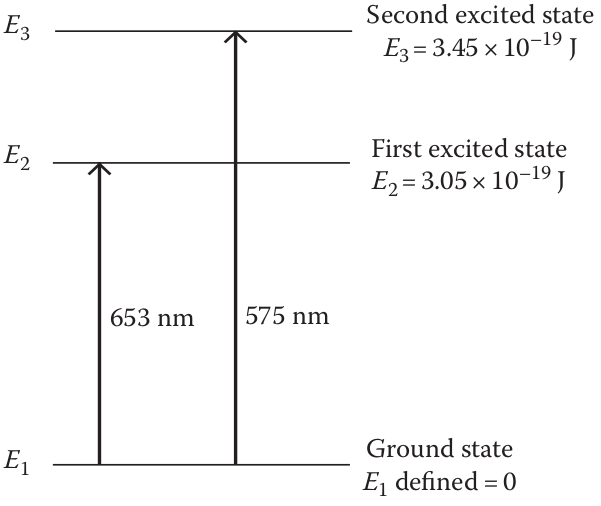
\includegraphics[width=0.5\textwidth]{2020-12-25_18-46.png}
    \caption{简单能级图}
    \label{fig:EnergyDia}
\end{figure}

图中显示两个激发态:一个对应蓝色玻璃吸收$653 nm$波长的光,另一个对应吸收$575 
nm$。玻璃不吸收蓝光,图中没有任何涉及到蓝光的能量状态。红光的吸收发生在$620$到
$750 nm$,黄光的吸收发生在$550$到 $590 nm$,如此类推。实验中,为什么分子吸收
光谱是宽频的呢?玻璃吸收可见光,归因于分子中价电子的激发,或者说电子跃迁。电子
跃迁比转动和振动需要更多的能量,转动$<$振动$<$电子。图\ref{fig:EnergyDia2}更
接近实际的能级图。
\begin{figure}[htpb]
    \centering
    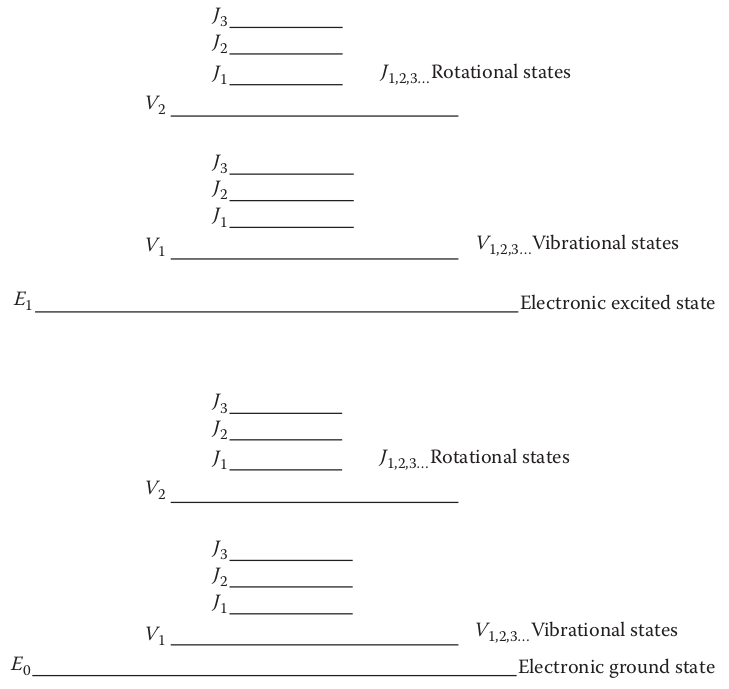
\includegraphics[width=0.55\textwidth]{2020-12-25_21-55.png}
    \caption{分子能级图,$E_{0,1,2,\dots}$表示各电子能级,$V_{1,2,3,\dots}$振动
    子能级,$J_{1,2,3,\dots}$为转动子能级}
    \label{fig:EnergyDia2}
\end{figure}
对于每一个电子态$E_n$都有许多转动和振动子能级。每一个子能级之间由很小的能量差异
,从一个能级$E_n$跃迁至另一个较高的能级,不是单一的能量,电子可以停留在
任意子能级上,从而导致是一个能量范围。所以,分子对红光的吸收,在一定的波长范围
内,而不是单一的、离散的波长。

激发态能量不稳定,分子或原子需要回到最低能量状态,并释放出能量,通常是以发光的
形式。激发态很短暂,在$10^{-9}$到$10^{-6} s$的范围内。

分子或原子吸收符合$\Delta E = h\nu = hc/\lambda$的辐射能时,便可绘制吸收光谱。
物质的吸收光谱展示了吸收的光的能量(频率或波长),以及在每个频率或波长下吸收
多少光。分子或原子的性质,决定在给定条能量下吸收光的量。物质的完整光谱包括
吸收的能量和吸收光的相应强度。纵轴表示强度变化,横轴表示频率或波长的变化。强度
与能量的关系图,就是我们通常说的光谱。聚苯乙烯的红外吸收光谱和苯的紫外吸收光谱
显示在图\ref{fig:example1}。
\begin{figure}[htpb]
    \centering
    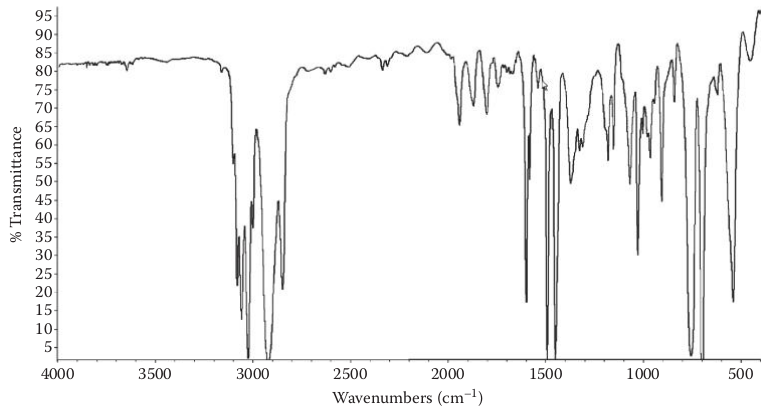
\includegraphics[width=0.85\textwidth]{2020-12-25_23-36.png}\\
    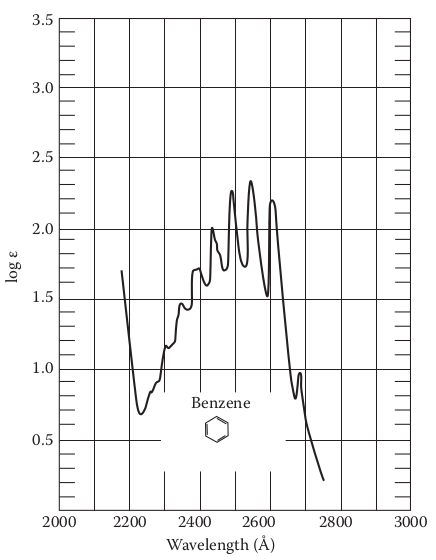
\includegraphics[width=0.65\textwidth]{2020-12-25_23-38.png}
    \caption{吸收光谱示例}
    \label{fig:example1}
\end{figure}

当处于激发态的原子或分子通过发射辐射能返回基态时,可获得发射光谱。发射光谱可
由形成激发态的许多不同方式产生。原子和分子不仅可以通过吸收电磁辐射来激发,而且
还可以通过原子和分子之间的碰撞而引起的能量转移,通过添加热能以及通过添加来自
放电的能量来激发。几种类型的发射光谱中使用了不同的激发方法,将在后面的章节中
详细讨论。在吸收电磁辐射激发后,原子或分子发射电磁辐射是一个特殊的术语。
这种发射称为发光。换句话说,如果将光用作激发的源,则将光的发射称为发光
(luminescence);如果使用其他激发源,则光的发射称为简单发射(emission)。

\section{原子和原子光谱}
核与绕核运动的电子构成原子。每一种元素都有特定的核电荷数,即电子数和质子数。
电子在不同的原子轨道运动,具有不同的能量,电子的能量态是量子化的。最低能量,
元素最稳定的电子构型称为基态。在无机化学中,我们已经学习基态原子电子构型,
遵循能量最低原理、保里不相容原理和洪特规则。例如,基态钠原子电子构型为
$1s^22s^22p^63s^1$;基态钾原子电子构型为$1s^22s^22p^63s^23p^64s^1$;
基态钒原子电子构型为$1s^22s^22p^63s^23p^64s^23d^3$,诸如此类。原子吸收光的能量
,外层(价)电子从基态跃迁至较高能量轨道,即能量高、不稳定的激发态。电子要从
激发态返回基态,电子放出能量。这个能量,在量上等于激发态和基态两个能级的差值。
该过程如图\ref{fig:2.5}所示。如果释放能量是以电磁辐射的形式,电子跃迁就满足
式(\ref{diffEnergy})和(\ref{diffEnergy2})
\begin{equation}
    \Delta E = E_{\text{final}} - E_{\text{initial}} = h\nu =
    \frac{hc}{\lambda}
    \label{eq:2.6}
\end{equation}
每种元素因其独特的电子构型,都有独特的所允许的电子能级。吸收或发射的光的波长,
是该元素特征属性。原子对辐射能的吸收,称为原子吸收光谱,将在后续章节学习。
\begin{figure}[htpb]
    \centering
    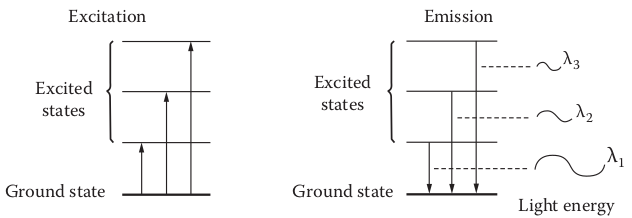
\includegraphics[width=0.8\textwidth]{2020-12-26_17-26.png}
    \caption{原子内能量跃迁}
    \label{fig:2.5}
\end{figure}

实际上,原子精确的能级图,是激发态原子的发射光谱。图\ref{fig:2.6}显示汞原子的
能级图。需要注意的是,原子没有转动和振动子能级。电子被激发到较高的激发态,
能量的变化非常明确,吸收(或发射时弛豫到基态)的波长可以认为是单色光。原子的
价电子跃迁所涉及的波长落在光谱的可见区和紫外区,该区域通常简称为UV/VIS。确定
所有元素的能级图,并提供原子吸收和发射的波长表,附录列出用于原子吸收光谱测量
的吸收波长。
\begin{figure}[htpb]
    \centering
    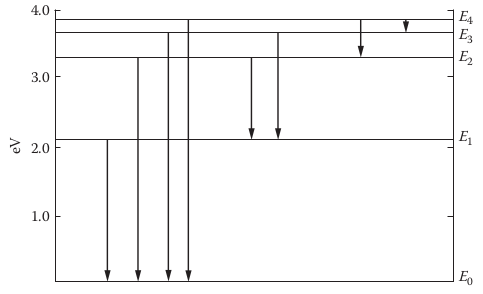
\includegraphics[width=0.65\textwidth]{2020-12-26_18-22.png}
    \caption{汞原子能级图}
    \label{fig:2.6}
\end{figure}

已知样品吸收或发射光的波长,可以对样品中存在元素进行定性鉴定。测量在给定波长
处吸收或发射的光的强度,可以给我们元素定量的信息。原子光谱法(吸收、发射和
荧光)灵敏度非常高,检测极限为$10^{-12}$到$10^{-15}$克。

原子有可能在X射线区域吸收更高能量的辐射。这样的吸收可能导致内壳(核)电子被
激发,随后发射X射线。此过程构成X射线荧光(XRF)光谱。
\section{分子和分子光谱}
与分子相关的能量状态,像原子一样,也被量子化。使用无线电波到紫外区域的辐射
来研究分子中允许状态之间跃迁的光谱方法非常强大。这些方法提供有关分子定性和
定量的信息,包括有关分子结构的详细信息。
\subsection{转动跃迁}
分子在空间中转动具有相关的转动能。分子可能仅以离散(量子化)的转动能态存在。
吸收适当的能量会导致从较低能量的转动状态过渡到较高能量的转动状态,其中分子
转动得更快。该过程引起转动吸收光谱。分子的转动能量取决于其角速度,该角速度
是可变的。转动能量还取决于分子的形状和重量分布,它们随键角的变化而变化。
尽管在\ce{O2}等双原子分子中形状的变化受到限制,但具有两个以上原子的分子
(例如己烷,\ce{C6H14})具有许多可能的形状,因此具有许多可能的转动能级。
此外,分子中原子中不止一个自然同位素的存在会产生新的一组转动能级。
碳就是这种情况,其中含碳分子中,小百分比原子的碳原子是\ce{^{13}C}而不是
\ce{^{12}C}
。因此,即使是简单的分子也具有复杂的转动吸收光谱。转动变化涉及的能量非常小,
每个分子约$10^{-24}J$。因此,吸收的辐射位于频谱的射频(RF)和微波区域。
由于所涉及的实验困难和所产生光谱的复杂性,在分析化学中尚未充分利用微波光谱法。
该技术仅限于气相,并且被射电天文学家用来检测星际云中的化学物质。
\subsection{振动跃迁}
\begin{figure}[htpb]
    \centering
    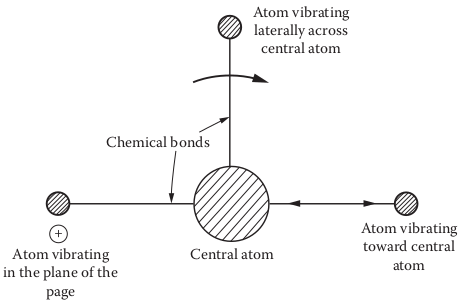
\includegraphics[width=0.7\textwidth]{2020-12-26_19-17.png}
    \caption{分子中成键原子可能的振动}
    \label{fig:2.7}
\end{figure}
可以将分子视为通过弹簧(化学键)连接在一起的一组重物(原子)。原子可以朝着
压缩和拉伸两个方向彼此振动,或者以各种角度彼此弯曲,如图\ref{fig:2.7}所示。
每个这种振动都具有与之相关的特征能量。量子化与分子振动相关的振动能态。分子的
振动能的变化与光谱的红外区域辐射能的吸收有关。虽然红外辐射的吸收会引起吸收
分子的振动发生变化,但振动能的增加通常还伴随着分子转动的增加。转动能级是振动
能级的子能级,如图\ref{fig:EnergyDia2}所示。因此,实际上,红外辐射的吸收对应
于分子中转动能和振动能变化的组合。由于具有两个以上原子的分子具有许多可能的
振动状态,因此红外吸收光谱很复杂,由多个吸收带组成。分子吸收红外辐射是光谱学
中最重要的技术之一。通过红外吸收光谱,可以推断出分子的结构,并且可以进行分子
的定性鉴定和样品分子组成的定量分析。
\subsection{电子跃迁}
当原子结合形成分子时,各个原子轨道结合形成一组新的分子轨道。在结合核的平面内,
沿着连接结合核的轴具有电子密度的分子轨道称为sigma($\sigma$)轨道。具有在键合核
平面之上和之下的电子密度的那些分子轨道称为pi($\pi$)轨道。$\sigma$和$\pi$轨道可
能有两种类型:成键轨道或反键轨道。成键轨道的能量低于相应的反键轨道。当将分子中
的电子分配给轨道时,最低能量的成键轨道首先被填充。有关分子轨道理论的综述,请
参阅无机化学。

在温度和压力的正常条件下,分子中的电子处于基态构型,填充了可用
的最低能量的分子轨道。吸收适当的辐射能会导致外部电子被提升为更高能量的激发态。
与原子一样,引起分子电子跃迁所需的辐射能位于可见光和紫外线区域。与原子一样,
分子的激发态没有基态稳定。分子将自发还原(弛豫)到发射UV/VIS辐射能的基态。
与原子不同,分子中的能量状态具有转动和振动子能级,因此当分子的电子被激发时,
振动和转动能通常会同时发生变化。总的能量变化是电子的、转动的和振动的能量转变。
分子具有许多可能的转动和振动状态,大量分子对UV/VIS辐射的吸收(每个分子的转动和
振动状态略有不同)会导致在很宽的波长范围内吸收,这称为吸收带。分子的UV/VIS吸收
光谱通常具有几个宽吸收带,与红外光谱相比非常简单。分子吸收和发射光谱可以用
于化学物种的定性鉴定。这项技术曾经是用于确定有机分子结构的主要方法之一,但
已被功能更强大且普遍使用的NMR、IR和MS替代。UV/VIS吸收光谱常用于样品分子组成的
定量分析。分子荧光光谱是一种灵敏度极高的方法,具有检测单个分子的能力。
\section{吸收定律}
光束的辐射功率$P$定义为单位面积内每秒的光束能量。相关的量是强度$I$,即每单位
立体角的功率。功率与强度都与光波振幅的平方有关,并且吸收定律可以用功率或
强度来表示。我们使用强度$I$,其它文献中,可能会看到用$P$的幂的形式。

\begin{figure}[htpb]
    \centering
    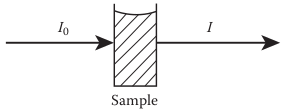
\includegraphics[width=0.4\textwidth]{2020-12-27_09-16.png}
    \caption{吸收示例}
    \label{fig:2.8}
\end{figure}

光通过吸收样品时,透射光的强度会降低。假设单色器光束(单一波长)强度为$I_0$,
样品吸收这一波长的辐射,如图\ref{fig:2.8}。透射光强度为$I$,$I_0 \geq I$。
如果样品不吸收辐射,$I = I_0$。吸光度$T$为
\begin{equation}
    T = \frac{I}{I_0}
    \label{2.7}
\end{equation}
透射率是入射光通过样品后的一个分数,取值范围为0到1。即使$I_0$发生变化,
$I/I_0$这一比例也会保持相对恒定。也就是说,$T$是不依赖实际强度$I_0$。研究
物质吸收的量,另一个物理量是吸光度$A$
\begin{equation}
    A=\log{\left(\frac{I_0}{I}\right)}
    =\log{\left(\frac{1}{T}\right)}=-\log{T}
    \label{2.8}
\end{equation}
没有光吸收,$I=I_0$,$A=0$。百分比透射率,$\% T$,等于$T\times 100$,百分比
吸光度,$\% A$,等于$100-\%T$,也常用于光谱中。
\begin{problem}
    假设有一水溶液吸收样品放置于底面边长为1 cm正方形的玻璃样品池中,如图
    \ref{fig:2.9}。光程$b$,入射光$I_0$强度为100,经过第一个样品池,有50\%的光被
    吸收,有50\%光透过。透射光$I_1$为50强度单位,所以,$\% T = 50$
    \begin{figure}[htpb]
        \centering
        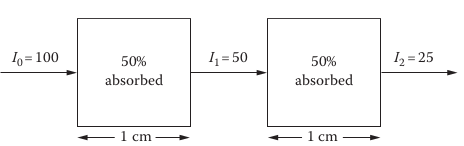
\includegraphics[width=0.75\textwidth]{2020-12-27_09-43.png}
        \caption{双样品吸收}
        \label{fig:2.9}
    \end{figure}
    \[
        \begin{array}{l}
            T = \frac{\% T}{100} = \frac{I_1}{I_0}\\
            T = \frac{50}{100} = 0.50
        \end{array}
    \]
    通过$T$计算吸光度
    \[
        A = -\log{T} = -\log{\left(0.50\right)} = 0.30
    \]
    第二个样品池放置相同的溶液,50\%的入射光被吸收,新的透射光$I_2$,25个强度
    单位,透过率
    \[
        T = \frac{I_2}{I_1}=\frac{25}{50}=0.50
    \]
    吸光度$A=-\log{0.50}=0.30$
\end{problem}
\begin{problem}
    现在我们将上例中,两个样品池背靠背放在一起,不考虑玻璃壁,光程看成2 cm。
    入射光$I_0$还是100个强度单位,经过吸收后,透射光$I$为25个强度单位。对于
    2 cm光程,$T=25/100=0.25$,$A=-\log{0.25}=0.60$。如果我们将三个样品池串联
    ,光程变为3 cm,透射光$I = 12.5$,$T=0.125$,$A=0.90$;四个样品池的情况
    为,$I=6.25$,$T=0.063$,$A=1.20$。绘制$I$与样品池个数曲线,见图
    \ref{fig:2.10}(a)所示,强度$I$随着光程长度的增加,显现指数下降。在吸光度
    相对于光程的图\ref{fig:2.10}(b)中,吸光度随着光程长度的增加,呈线性
    增加。对比(a)(b)两图,线性方程比指数方程更容易分析和整理数据,通过简单
    计算就能得到线性关系中的斜率,进一步获得横纵轴物理量之间的关系。光程长度
    与吸光度成正比,由P. Bouguer (1729)和J. Lambert (1760)发现。
    \begin{figure}[htpb]
        \centering
        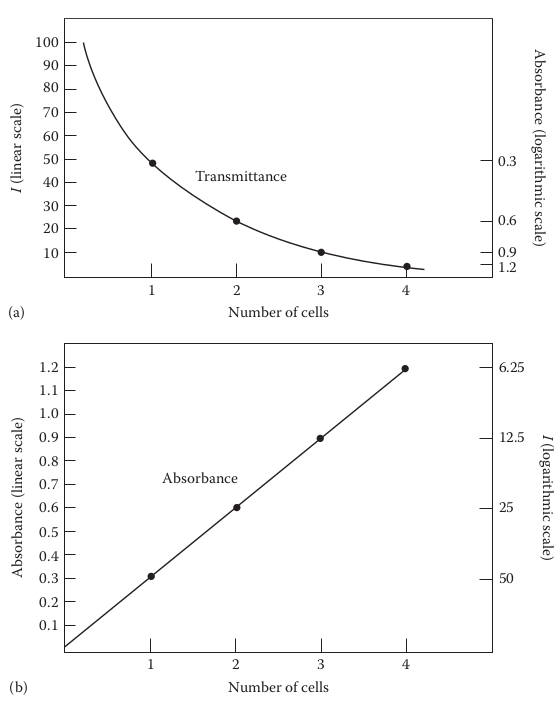
\includegraphics[width=0.85\textwidth]{2020-12-27_12-12.png}
        \caption{光程长对吸收的影响}
        \label{fig:2.10}
    \end{figure}
\end{problem}

保持光程长(样品池)不变,改变试样浓度,$I$、$A$与浓度之间的关系,与上例相同。
吸光度与浓度呈线性,于是我们得到
\begin{equation}
    A = \varepsilon l c
    \label{2.9}
\end{equation}
$l$是光程长度,单位为cm,$c$是样品浓度,单位为mol/L。$\varepsilon$是摩尔吸光
系数,对于给定物质,在特定波长下,该值为一常数。Beer在1852年发现浓度与吸光度
之间成正比关系。

综合吸光度、样品浓度、光程长度和摩尔吸光系数之间的关系,{\bf Beer-Lambert
-Bouguer}定律,简称为{\bf Beer}定律,从$A=-\log{T}$
\begin{equation}
    \varepsilon l c = -\log{T}
\end{equation}
\begin{equation}
    -\log{\left(\frac{I}{I_0}\right)}=\varepsilon l c 
\end{equation}
\begin{equation}
    \log{\left(\frac{I_0}{I}\right)}=\varepsilon l c 
\end{equation}
\begin{equation}
    \frac{I_0}{I}=10^{\varepsilon l c }
\end{equation}
\begin{equation}
    \frac{I}{I_0}=10^{-\varepsilon l c }
\end{equation}

根据观察到的实验事实,比尔定律从数学上表明,如果入射光的路径长度和波长保持
恒定,则$A$与吸收物质的浓度之间存在线性关系。这在分析光谱学中是极其重要的
关系。它通过定量测量吸收的辐射量,为定量分析样品中分析物的浓度奠定了基础。
辐射强度的定量测量称为光谱法。所有定量光学吸收光谱法(红外吸收光谱法,
AAS,UV/VIS吸收光谱法等)均满足比尔定律。
\subsection{Beer定律的偏差}
对于均质样品,通常在低分析物浓度下遵循Beer定律。当浓度小于约0.01 M时,大多数
吸收物质的吸光度与浓度成正比。

高浓度的分析物通常会出现线性偏差。在高浓度下有几种偏离线性的可能原因。
在溶液中浓度较低时,分析物将被视为溶质。随着溶质浓度的增加,分析物分子可能会
通过分子间吸引力(例如氢键和其他范德华力)开始相互影响。这种相互作用可能会改变
分析物的吸收率,从而随着浓度的增加而产生非线性响应。在极高的浓度下,溶质实际上
可能成为溶剂,从而改变了溶液的性质。如果分析物与其他物质处于化学平衡状态,
例如溶液中的弱酸或弱碱,则分析物浓度的变化可能会改变平衡(Le Chatelier原理)。
当溶液稀释或浓缩时,这可能反映在明显偏离比尔定律的地方。

如果样品散射入射辐射,则可能会出现另一种背离Beer定律的来源。溶液必须不含漂浮
的固体颗粒,并且在测量前通常要过滤。高分析物浓度时发生非线性的最常见原因是
光太少而无法吸收。在较低的分析物含量下,浓度加倍会使吸收的光量增加一倍,
例如从25\%增至50\%。如果已经吸收了99\%的光,则将浓度增加一倍仍将使吸收的剩余
光量增加一倍,但是变化仅从99\%到99.5\%。这导致曲线在高吸收率时变得平坦。

从式\ref{2.8}可以看出,$A = \log\left(I_0/I\right)$。如果$I_0 = 100$且
$A = 1.0$,则$I =10$。仅透射初始辐射强度的10\%。强度的其他90\%被样品吸收。
如果$A = 2.0$,则$I = 1.0$,表明99\%的入射光被样品吸收。如果$A = 3.0$,则
吸收99.9\%的入射光强度。正如我们将看到的,随着$A$的增加(或$I$的减少),$A$的
测量误差也随之增加。实际上,吸光度值小于或等于1.0符合Beer定律。
\section{数据处理方法}
建立我们测量的信号(例如吸光度)与已知分析物浓度之间关系。一旦建立了这种关系,
就可以通过测量未知信号来计算未知样品中分析物的浓度。随后讨论的方法不仅适用于
光谱测量,而且适用于大多数分析仪器方法。从历史上看,数据是通过手动读取仪表或
用直尺测量峰高,并将所有数字转录到实验室笔记本中来手动收集的。
信号和浓度之间的关系在座标纸上手动绘制。现代仪器具有软件包,这些软件包可以
使数据点统计到最适合的直线或曲线,并在计算机屏幕上显示结果并将其发送到打印机。
计算机化的数据收集和处理功能大大减少了抄写错误,将错误的图形复制到笔记本中。
线性回归和其他曲线拟合方法的使用,在拟合方程式和从方程式计算出的样品结果中
提供了更高的准确性和精确度。
\subsection{标准曲线法}
为了使用比尔定律确定未知物中的分析物浓度,必须确定给定波长下的吸光度与分析物
浓度之间的关系。已知浓度分析物的溶液称为标准溶液。对于某些类型的分析,标准液
可以采用固体或气体形式。

必须使用高纯度材料准确地制备标准品,以便尽可能准确地知道分析物的浓度。准备
涵盖适当浓度范围的一系列标准溶液。标准溶液应包括一种不添加分析物的溶液;该标准
溶液中分析物的浓度为零。该溶液称为试剂空白,用于解释由于溶剂和用于制备样品的
其他试剂中的杂质而引起的吸光度,它还说明了仪器基线。试剂空白和每种标准品的
吸光度为测量。在执行任何计算之前,将从其他标准溶液的吸光度中减去试剂空白
的吸光度。从中减去空白吸光度的吸光度称为“校正吸光度”。在$y$轴上校正吸光度
与$x$轴上标准品的已知浓度作图。这种图曾经在座标纸上手动构建;现在,绘图是由
计算机软件完成的。这种典型标准曲线如图\ref{fig:2.11}所示。该标准曲线显示了
IR区域中在石油中发现的正十六烷,\ce{CH3(CH2)14CH3}(在石油中发现的碳氢化合物)
在$3.41\mu m$处的吸光度与正十六烷在四氯乙烯,\ce{C2Cl4},中的溶液浓度之间的
关系。这种对正十六烷溶液在$3.41\mu m$处的吸光度的测量是一种用于确定水,土壤
和其他环境样品中石油污染的方法,因为大多数碳氢化合物都在该波长下吸收。依据
Beer定律来测量未知样品中的石油烃。它用于测量漏油,非法倒油和地下储油罐泄漏
造成的环境污染。
\begin{figure}[htpb]
    \centering
    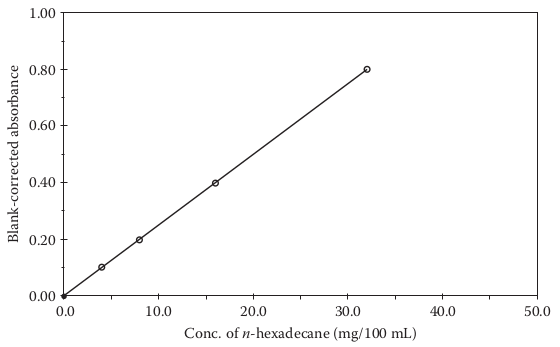
\includegraphics[width=0.75\textwidth]{2020-12-27_20-50.png}
    \caption{标准曲线示例}
    \label{fig:2.11}
\end{figure}
\begin{table}[htbp]
    \centering
    \caption{石油红外吸光度校正数据}
    \label{tab:2.4}
    \begin{tabular}{ccc}
        \hline
        正十六烷浓度 & $3.41\mu m$吸光度  &  修正吸光度\\
        \hline
        0.0  &  0.002   &  0.000  \\
        4.0  &  0.103   &  0.101  \\
        8.0  &  0.199   &  0.197  \\
        16.0  &  0.400   &  0.398  \\
        32.0  &  0.804   &  0.802  \\
        \hline
    \end{tabular}
\end{table}

表\ref{tab:2.4}给出每种标准品的浓度值以及测量和校正的吸光度。从图\ref{fig:2.11}
可以清楚地看出,此测量的吸光度与浓度之间的关系遵循比尔定律,因为该图产生一条
直线($y = mx + b$,其中$y$是吸光度,$x$是浓度)。绘制点后,将通过数据点
拟合最佳直线。最合适的直线拟合的方法是线性回归(线性最小二乘法)。当然,也可以
从标准曲线上直观观察到,与给定吸光度相对应的浓度。但为了进行精确工作,必须
确定最佳拟合直线方程式。

对表\ref{tab:2.4}中的数据进行拟合,可以得到确定的Beer定律关系式:
$A=0.0250 c - 0.001$,这里$c$是正十六烷的浓度,单位为mg/100 mL。根据标准曲线
方程,可以确定任何测量的吸光度的浓度。例如,根据美国EPA方法8440制备了未知的
受污染土壤样品,并测量样品溶液的吸光度为0.302,因此,修正后的吸光度为
$0.302 - 0.002 = 0.300$。从标准曲线中,我们可以观察到,这相当于12.0 mg
正十六烷/100 mL的浓度。精确的浓度可以通过线性回归方程计算得出,11.96 mg/100 mL
,或12.0 mg/100 mL(四舍五入三位有效数字)。

\begin{figure}[htpb]
    \centering
    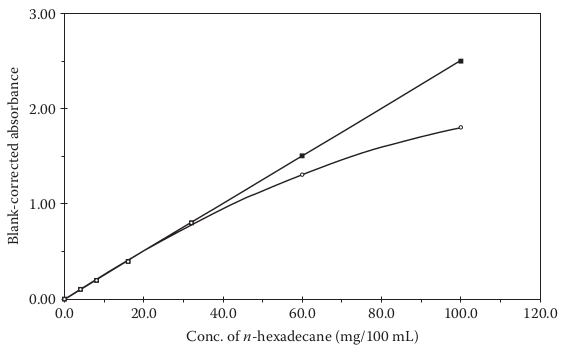
\includegraphics[width=0.85\textwidth]{2020-12-28_22-56.png}
    \caption{校正曲线}
    \label{fig:2.12}
\end{figure}
\begin{table}[htbp]
    \centering
    \caption{石油红外吸光度校正数据(高浓度)}
    \label{tab:2.5}
    \begin{tabular}{ccc}
        \hline
        正十六烷浓度 & $3.41\mu m$吸光度  &  修正吸光度\\
        \hline
        0.0  &  0.002   &  0.000  \\
        4.0  &  0.103   &  0.101  \\
        8.0  &  0.199   &  0.197  \\
        16.0  &  0.400   &  0.398  \\
        32.0  &  0.804   &  0.802  \\
        60.0  &  1.302   &  1.300  \\
        100.0  &  1.802   &  1.800  \\
        \hline
    \end{tabular}
\end{table}

假设除了表\ref{tab:2.4}列出的数据之外,我们还制备了正十六烷的标准溶液,其中包含
60.0 mg/100 mL和100.0 mg/100 mL两种浓度,吸光度数据如表\ref{tab:2.5}所示。
图\ref{fig:2.12}画出其它点,用空心圆表示,并标出了原始浓度。显然,在高浓度下,
偏离Beer定律,这些点不再是直线关系,测得的吸光度低于遵循Beer定律情况下的
吸光度。这说明,为什么将标准曲线外推延展到测量标准物的范围之外,从来不是一个
好主意。如果我们有一个吸光度为1.30的样品(60.0 mg/100 mL),并且使用我们原来
的标准曲线外推到更高的吸光度,图\ref{fig:2.12}黑色方块所示,那么我们将计算出
51.9 mg/100 mL的试样浓度,错误的降低了。如果吸光度高于最高 线性标准吸光度(
在此例中是$A=0.802$),最好的办法是将样品稀释。将60.0 mg/100 mL的样品进行稀释
十倍。
\subsection{标准加入法}
这种方法将已知量的分析物直接添加到样品中,其中包含未知量的分析物。由于添加
分析物而导致信号的增加(例如,吸光度,发射强度)使我们能够计算未知物中的
分析物量。为了使这种方法有效,分析物浓度和信号之间必须存在线性关系。

如果未准备好合适的外部校准曲线,则通常使用标准加入法。可能没有时间准备校准标准
品,例如,在医院紧急情况下,可能有必要快速测量患者血清中的钠。由于样品基质的
复杂性或缺少有关样品的足够信息,可能无法准备一套有效的校准标准。当流程中出现
问题时,行业通常需要分析``神秘''样本。当样品基质中存在某些类型的干扰时,非常有
用。 标准加入法允许我们通过在存在干扰的情况下执行校准来获得准确的结果,而不会
消除干扰。当仅需分析一个样品且外部标准品的制备效率低下时,通常会使用此方法。

标准加入法典型使用示例是通过原子发射光谱法测定未知成分的工业废水中的钠。提取
植物流的代表性样品,并分成四个等分试样,每个等分试样为100 mL。第一份等分试样
未经处理;这称为``不添加''或``零添加''样本。向第二等分试样中,以不明显改变体积
的方式向100 mL样品中添加100 $\mu$g \ce{Na}。这可以通过向样品中添加10 $\mu$L体积
的10000 ppm \ce{Na}溶液来完成。10000 ppm \ce{Na}溶液包含10000 $\mu$g \ce{Na}/mL
,因此下式所示,每10 $\mu$L部分包含100 $\mu$g \ce{Na}
\[
    \left(\frac{10000\quad \mu g\quad Na}{mL\quad solution}\right)
    \left(\frac{1\quad mL}{1000\quad \mu L}\right)
    \times 10\quad \mu L = 100\quad \mu g\quad Na
\]
现在第二个样品等分试样包含额外的1.0 ppm \ce{Na},因为100 $\mu$g \ce{Na}/100 mL
等于1.0 ppm \ce{Na}。向第三等分试样中,添加0.020 mL的10000 ppm \ce{Na}溶液;
现在,第三个包含额外的2.0 ppm \ce{Na}。在第四等分试样中,添加0.030 mL的10000
 ppm \ce{Na}溶液会在样品等分试样中产生额外的3.0 ppm \ce{Na}。由于添加了\ce{Na}
 溶液而引起的最大体积变化仅为0.03\%,数量可忽略不计。重要的是不要更改等分试样
 的体积,因为体积的变化会引起浓度-信号关系的变化。所有未处理的等分试样和
 已添加的等分试样必须具有相同的成分,否则标准加入法将不会产生准确的结果。
表\ref{tab:2.6}列出了添加的\ce{Na}的浓度和样品的等分试样编号。使用火焰俄歇
电子能谱(AES)或火焰光度计在589.0 nm的钠发射线上测量四个样品等分试样中
每一个的发射强度。测得的强度也列在表\ref{tab:2.6}中。此外,在没有样品的情况下
测量火焰的发射强度。这可测量“背景辐射”,即来自火焰的正信号,而不是样品引起的。
必须从样品强度中减去背景发射信号,就像我们前面所讨论的那样减去试剂空白,
才能获得表\ref{tab:2.6}中所示的校正强度。
 \begin{table}[htbp]
     \centering
     \caption{标准加入法}
     \label{tab:2.6}
     \begin{tabular}{lccc}
         \hline
         样品份 & 发射强度 & 修正强度  & \ce{Na}加入量(ppm)\\
         \hline
         1  &  2.9  & 2.4  &  0.0  \\
         2  &  4.2  & 3.7  &  1.0  \\
         3  &  5.5  & 5.0  &  2.0  \\
         4  &  6.8  & 6.3  &  3.0  \\
         背景  &  0.5  & 0.0  &    \\
         \hline
     \end{tabular}
 \end{table}
 \begin{figure}[htpb]
     \centering
     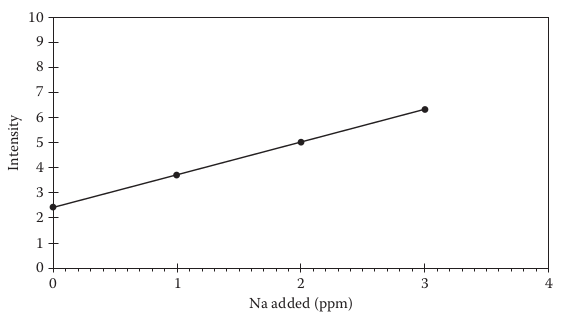
\includegraphics[width=0.85\textwidth]{2020-12-29_22-04.png}
     \caption{典型标准加入法曲线}
     \label{fig:2.13}
 \end{figure}

修正后的发射强度,相对于添加\ce{Na}浓度绘制曲线(图\ref{fig:2.13}。从图中可以
看出,所添加的浓度与信号之间的关系在所检测范围内,呈线性关系。
$\Delta I_{\text{emission}}/\Delta ppm \text{Na}$比值为斜率,通过线性回归
计算得出的。每1.0 ppm \ce{Na}加入,发射光强度增加1.3倍。未处理\ce{Na}样品浓度
的计算式为
\[
    \text{ppm Na} = \frac{R}{slope} = R(slope)^{-1}
\]
此处,$R$是第一份样品修正后的测量强度,$slope$为斜率。我们例子中,\ce{Na}
浓度为
\[
    \text{ppm Na}=2.4 \text{ initensity units}
    \times\frac{1.0 \text{ ppm Na}}{1.3 \text{ intensity units}}
    = 1.85 \text{ ppm}
\]
或者,可以使用确定的线性回归方程将标准加入曲线外推到$x$轴负方向上的截矩。样品
中\ce{Na}的浓度等于$x$轴截矩的绝对值。对于表\ref{tab:2.6}中数据,外推如图
\ref{fig:2.14}所示。$x$负方向截矩为$-18.5$;因此,样品中\ce{Na}的浓度为
$|-1.85 \text{ ppm}| = 1.85\text{ ppm}$
\begin{figure}[htpb]
    \centering
    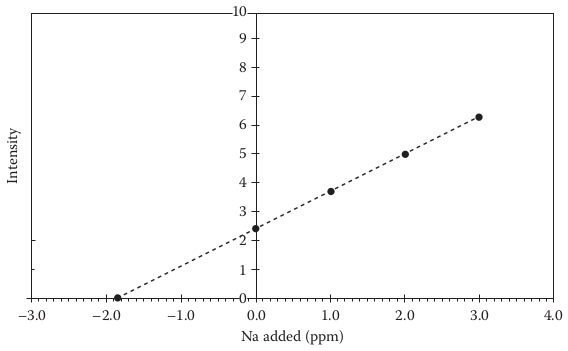
\includegraphics[width=0.85\textwidth]{2020-12-30_23-59.png}
    \caption{标准加入法}
    \label{fig:2.14}
\end{figure}
标准加入法是非常强大的工具,可在无法准备外部校准曲线时获得准确的分析结果。
在某些情况下,即使存在干扰物质的情况下,也可以获得准确的结果。此方法无法校正
背景发射或背景吸收或其他光谱干扰。

如果样品量有限(可能非常适合患者的血清),则可以使用单点标准添加技术。通过
火焰原子发射测定血清中钠的技术,测量样品的发射强度,然后添加已知浓度的\ce{Na},
而又不会明显改变样品的体积。测量添加样品的发射强度,以及火焰背景。发射信号与
浓度成正比,可以写成
\[
    \frac{I_{\text{unknown}}}{I_{\text{added}}} =
    \frac{\text{ppm Na}_{\text{unknown}}}
    {\text{ppm Na}_{\text{unknown}} + \text{ppm Na}_{\text{added}}}
\]
$I_{\text{unknown}}$是原始样品校正强度,$I_{\text{added}}$是添加\ce{Na}的样品
校正强度,$\text{ppm Na}_{\text{added}}$加入\ce{Na}的浓度。
例如,血清样品的测量给出2.4强度单位的校正强度。将足够的钠添加到血清样品中,使
浓度增加3.0 ppm,校正强度为6.3,设$x=\text{ppm Na}_{\text{unknown}}$,
\[
    \frac{3.7}{6.3}=\frac{x\text{ ppm}}{(x + 3.0)\text{ ppm}}
\]
解得
\[
    x = 4.3\text{ ppm Na}
\]
尽管样品有限,使用单点添加,可能的情况下至少两个添加,以确定分析方法的线性
范围。
\subsection{内标法}
内标法是添加到所有样品,空白和标准溶液中的已知量的非分析元素或化合物。
使用内标法进行校准是一种使用来自内部标准元素或化合物的信号来校正分析中干扰
的技术。通过内标法可以补偿多种误差源,从而提高分析的准确性和精确度。为确定
分析物A,选择样品中不存在的内标S。将相同浓度的S添加到所有样品,标准溶液和空白
样品中。测量归因于A和S的信号。计算归因于分析物A的信号与归因于内标S的信号的
比率。将信号比相对于标准液中的浓度比作图。通过线性回归可得到校准曲线的方程,
该方程应为线性以获得最佳结果。该公式允许通过测量样品中A和S的信号来计算
任何未知样品中的浓度比A/S,浓度与信号之间的关系可以表示如下:
\[
    \frac{\text{Concentration ratio(A/S) in sample}}
    {\text{Concentration ratio(A/S) in standard}} =
    \frac{\text{Signal ratio(A/S) in sample}}
    {\text{Signal ratio(A/S) in standard}}
\]
内标法广泛适用于光谱、色谱、质谱和其它仪器分析方法中。可以校正样品制备过程中
分析物的损失,分析过程中仪器中机械或电气的“漂移”,由于蒸发和其他类型的干扰
引起的体积变化。通常必须谨慎选择内标,以使内标的化学和物理行为与分析物相似。
内标不得与分析物发生化学和物理相互作用。任何影响分析物信号的因素,都应以
相同的方式影响内标物的信号。即使绝对信号发生变化,两个信号的比率也将保持
恒定。与不使用内标相比,这提供了更高的准确性和精确度。

通过电感耦合等离子体质谱仪(ICP-MS)对饮用水中的铅进行测定,内标如何纠正
诸如“仪器漂移”之类的问题,即一段时间内信号的变化。监视Pb-208同位素($^{208}$Pb
)的信号以确定铅。制备两种铅校准标样,每种标样均含10.0 ppb铅。一种标准品还
包含20.0 ppb的铋作为内标。\ce{Bi}信号与Pb-208信号一起在Bi-209同位素处测量。
一天中对这两种标准品进行了多次测量,结果信号列于表\ref{tab:2.7}。
从表\ref{tab:2.7}可以看出,
\ce{Pb}和\ce{Bi}的信号在一天中波动;例如,这种波动可能是由于仪器的电线电压
变化引起的。但是,如最后一栏所示,分析物信号与内标信号的比率在一天中保持恒定。
如果在上午8点不使用内标对ICP-MS进行校准,则在下午1点运行的样品会给出错误的
高Pb浓度,因为给定数量的铅的信号增加了2.5倍。在下午3点,样本将比真实值高大约
30\%。如果已将20.0 ppb \ce{Bi}添加到所有标准液和样品中,则Pb信号/Bi信号之比
将保持恒定,并确定准确的铅浓度。例如,ICP-MS在8 AM校准为仅含10.0 ppb \ce{Pb}的
标准溶液。对于10.0 ppb \ce{Pb},获得的信号为12050个计数。这是校准因子:
12050个计数/10.0 ppb铅。测量含有10.0 ppb \ce{Pb}和20.0 ppb \ce{Bi}的第二溶液;
如表\ref{tab:2.7}所示,铅的计数为12050(与标准值相同),而铋的计数为60000。
全天测量添加了20.0 ppb \ce{Bi}作为内标的饮用水样品。表\ref{tab:2.8}给出了
获得的信号。上午八点,铅信号为6028,没有内标物的情况下,使用校正因子计算水中
铅浓度
\begin{table}[htbp]
    \centering
    \caption{内标法校正}
    \label{tab:2.7}
    \begin{tabular}{lccc}
        \hline
        \multirow{2}*{测量时间} & 信号  &   信号  &  比率\\
        & 10 ppb Pb, m/e = 208 & 20 ppb Bi, m/e = 209 & Pb/Bi \\
        \hline
        上午八点 &  12050 & 60000  & 0.2008 \\
        上午十点 &  12100 & 60080  & 0.2013 \\
        下午一点 &  30000 & 149200  & 0.2010 \\
        下午三点 &  15750 & 78400  & 0.2009 \\
        \hline
    \end{tabular}
\end{table}
\[
    \begin{array}{rcl}
\text{ppb Pb in sample}&=&(6028)\dfrac{10.0\text{ ppb Pb}}{12050}\\
    \text{ppb Pb in sample}&=&5.00\text{ ppb Pb}
\end{array}
\]
这是样品中铅的真实值。使用相同方法,计算铅信号其余浓度,结果显示在表
\ref{tab:2.8}的第三列。下午一点和三点数据明显出现错误,归因于仪器“漂移”。
例如,下午一点的样品信号15010。使用铅校正因子计算浓度:
\[
    \begin{array}{rcl}
\text{ppb Pb in sample}&=&(15010)\dfrac{10.0\text{ ppb Pb}}{12050}\\
    \text{ppb Pb in sample}&=&12.5\text{ ppb Pb}
\end{array}
\]
仪器漂移的百分误差为:
\[
    \begin{array}{rcl}
    \text{\% Error}&=&\dfrac{\text{Measured value}-\text{True value}}
    {\text{True value}}\times 100 \\
    \text{\% Error}&=&\dfrac{12.5-5.00}{5.00}\times 100\\
    \text{\% Error}&=&+150\\
\end{array}
\]
如果使用内标\ce{Bi},内标校正因子,即Pb/Bi比率为:
\[
    10.0\text{ ppb Pb}=\dfrac{12050\text{ counts Pb}}{60000\text{ counts Bi}}
    =0.2008
\]
上午八点的样品,包含\ce{Bi}内标物,数据显示在表\ref{tab:2.8}。Pb/Bi比率为
$6028/60010=0.1004$,得到样品中铅浓度为:
\[
    \begin{array}{rcl}
        \text{ppb Pb in sample}&=&(0.1004)\dfrac{10.0\text{ ppb Pb}}{2.008}\\
        \text{ppb Pb in sample}&=&5.00\text{ ppb Pb}\\
    \end{array}
\]
\begin{table}[htbp]
    \centering
    \caption{有无内标水中铅的测定}
    \label{tab:2.8}
    \begin{tabular}{lccccr}
        \hline
        \multirow{2}*{测量时间} & \ce{Pb}计数 & ppb \ce{Pb} & \ce{Bi}计数 & 
        \multirow{2}*{Pb/Bi比率} & ppb \ce{Pb} \\
        & m/e = 208 & 无内标 & m/e = 209 & & 有内标 \\
        \hline
        上午八点 &  6028 & 5.00  & 60010 & 0.1004  & 5.00 \\
        上午十点 &  6063 & 5.03  & 60075 & 0.1009  & 5.02 \\
        下午一点 &  15010 & 12.5  & 149206 & 0.1006 & 5.01 \\
        下午三点 &  7789 & 6.46 & 78398  & 0.0994 & 4.95 \\
        平均值 &&7.25 &&&4.99\\
        标准差&&3.57&&&0.33\\
        相对标准差&&49.2&&&0.60\\
        真实值&&5.00&&&5.00\\
        误差&&45.0&&&$-0.2$\\
        \hline
    \end{tabular}
\end{table}
这与没有内标的结果相同。如果全天的样品内标的比率相同,仪器漂移的结果被修正。
例如,下午一点,\ce{Pb}为15010,\ce{Bi}为149206。这明显比上午八点高出很多,
但Pb/Bi的比率$15010/149206=0.1006$,铅的浓度为:
\[
    \begin{array}{rcl}
        \text{ppb Pb in sample}&=&(0.1006)\dfrac{10.0\text{ ppb Pb}}{2.008}\\
        \text{ppb Pb in sample}&=&5.01\text{ ppb Pb}\\
    \end{array}
\]
百分误差为:
\[
    \begin{array}{rcl}
        \text{\% Error}&=&\dfrac{5.01-5.00}{5.00}\times 100\\
        \text{\% Error}&=&0.2\\
\end{array}
\]
对于仪器分析来说,0.2\%的误差非常理想。

对比没有使用内标物的下午一点12.5 ppb的铅含量,尽可能的使用内标法是正确选择。
\subsection{Beer定律相关误差}
所有的光谱测量都有随机误差,直接影响准确度和精确度。光谱分析中最常见的随机
误差是仪器的“噪音”。噪音,归因于仪器光源的不稳定、检测器的不稳定、光路上样品
位置的变化,这些综合影响。误差是随机的,不能被消除。仪器辐射强度误差直接导致
使用校正曲线和Beer定律时浓度测量误差。

我们可以评估仪器噪音引起的随机误差对透过率测量的影响。以下讨论适用于光源强度
较低或检测器灵敏度较低的区域的UV/VIS和热检测器噪音较大的IR。根据Beer定律,
可以看出:
\begin{equation}
    \frac{\Delta c}{c} = \frac{0.434\Delta T}{T \log T}
    \label{2.15}
\end{equation}
其中,$\Delta c/c$浓度相对误差;$\Delta T$透过率测量误差。
\begin{definition}{推导过程}{beer}
\[
  -\log T = \varepsilon l c
\]
两边求导数
\[
  d(-\log T) = d(\varepsilon l c)
\]
等号左边$T$看作变量,右边$c$看作变量
\[
  -\frac{1}{x\ln 10}dT = \varepsilon l dc
\]
将$\varepsilon l = -\frac{\log T}{c}$代入,得
\[
  -4.303\frac{dT}{T} = -\log T \frac{dc}{c}
\]
\[
  \frac{\Delta c}{c} = \frac{4.303\Delta T}{T \log T}
\]
\end{definition}
可以从大量($n>20$)相同溶液的重复测量估算$\Delta T$的值。假设在$T$的测量中,
存在1\%的恒定误差,或者说$\Delta T=0.01$,可以使用式\ref{2.15}计算浓度的
相对误差,表\ref{tab:2.9}给出在该假定恒定误差下,各透过率测量中浓度的相对误差
。当$T$非常低或非常高的时候,浓度相对误差很大。当使用Beer定律,分析物的
浓度非常低(即透过率高),还是分析物浓度非常高(透过率低),都会导致重大误差。
\begin{table}[htbp]
    \centering
    \caption{相对浓度误差(1\%的仪器误差)}
    \label{tab:2.9}
    \begin{tabular}{lc}
        \hline
        透过率($T$) & 相对浓度误差($\Delta c/c$)$\times 100$(\%)\\
        \hline
        0.02 & 12.8\\
        0.08 & 4.9 \\
        0.15 & 3.5 \\
        0.30 & 2.8 \\
        0.37 & 2.7 \\
        0.45 & 2.8 \\
        0.65 & 3.6 \\
        0.80 & 5.6 \\
        0.97 & 33.8\\
        \hline
    \end{tabular}
\end{table}
\begin{figure}[htpb]
    \centering
    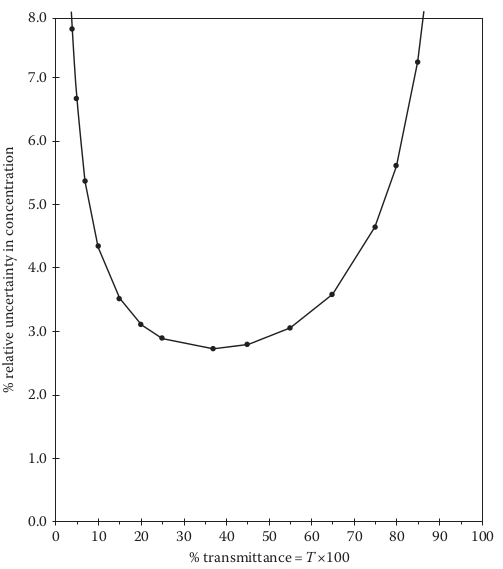
\includegraphics[width=0.75\textwidth]{2020-12-31_20-11.png}
    \caption{浓度测量的相对不确定性}
    \label{fig:2.15}
\end{figure}

我们可以将表\ref{tab:2.9}中的相对误差数据绘制为透过率的函数。结果如图
\ref{fig:2.15}所示。从该图可以看出,最小相对误差出现在$T = 0.37$,尽管
在15\%--65\%T的范围内可以获得令人满意的结果。该范围对应$于0.82 - 0.19$。为了
获得最大的定量吸收测量准确度,建议从吸光度在0.82至0.19之间的样品中确定浓度。
浓度过高的样品($A> 0.82$)应稀释以使其吸光度值低于0.8。太稀的样品
($A < 0.19$)应通过蒸发或溶剂萃取进行浓缩。如果无法更改样品溶液,分析人员
必须意识到,使用具有上述限制的仪器时,非常稀或非常浓的样品的相对误差会很大。

现代UV/VIS光谱仪通常受“shot noise”限制在光子检测器中电子穿越结。
在这种情况下,由于不确定的仪器误差而引起的相对不确定图与图\ref{fig:2.15}有
很大不同。对于高质量,shot noise受限的仪器,当A值非常低(\%T高)时,相对误差
会很高,但是从0.2到2.0以上的吸光度值具有大约相同的低($<1\%$)相对不确定度。
换句话说,由于仪器组件的改进,现代光谱仪比旧的光谱仪更加精确。

绘制光谱数据的另一种方法是使用Ringbom方法,其中横轴是浓度的对数,纵轴是
(100-%T)。所得的S形曲线称为Ringbom图。图\ref{fig:2.16}显示锰作为高锰酸根
离子吸收的Ringbom图。Ringbom图显示分析误差最小的浓度范围。这是曲线的陡峭部分,
斜率几乎是线性的。该图还可以评估在任何浓度水平下的准确度。根据Beer定律,可以
证明对于1\%的透射率误差,相对分析误差的百分比为
\begin{equation}
    \frac{\text{\% relative analysis error}}{\text{1\% transmittance error}} =
    \frac{100 \Delta c/c}{1} = \frac{230}{\Delta T/\Delta \log c}
    \label{2.16}
\end{equation}
因为数量($\Delta T/\Delta \log c$)是曲线的斜率,所以曲线上任意点每1\%的
透过率误差的相对分析误差等于230除以该点的斜率。可以通过在所需浓度下构建曲线的
切线来确定斜率。对于$x$的10倍差异,计算$y$的差异。该值除以230,即每1\%透射率
误差的相对分析误差百分比。例如,在图\ref{fig:2.16}中标记为A的两个点之间的斜率
是通过绘制切线来确定的,该切线穿过浓度2和20 ppm(变化10倍)。图中的$y$值在
2 ppm时为9\%,在20 ppm时为90\%。$y$值之差为$90 − 9 = 81$;因此,
$230/81 = 2.8$。在此范围内,相对分析误差为2.8\%。其他范围及其各自的误差在
图\ref{fig:2.16}左上方的插入框中显示。当然,与手动绘制切线相比,
使用计算机可以更准确地完成此计算。
\begin{figure}[htpb]
    \centering
    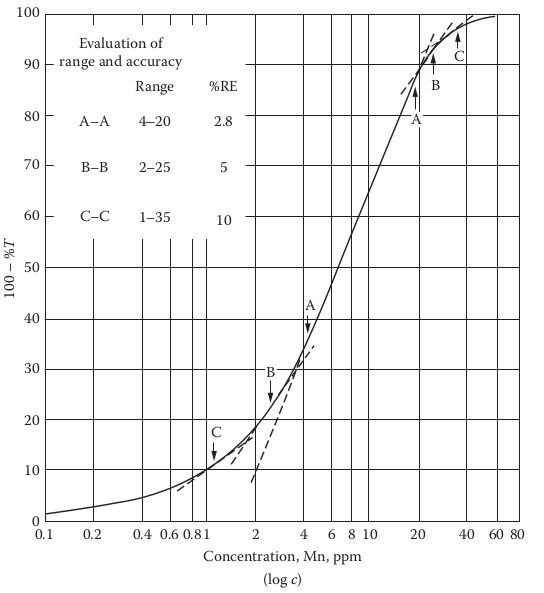
\includegraphics[width=0.75\textwidth]{2020-12-31_20-55.png}
    \caption{Ringbom图}
    \label{fig:2.16}
\end{figure}

Ringbom图的实际应用是确定浓度范围,在该范围内相对分析误差百分比不会超过指定值。
这种限制通常是为工业分析设置的,其中基于光谱测量结果为产品成分的上限和下限
建立了“好”产品的规格。超出这些规格的产品将被视为不符合要求而被拒绝。

对Ringbom图的解释得出的结论与我们从图\ref{fig:2.15}得出的结论相同。误差最低,
约为$100 - \% T = 63$或$37\% T$。每1\%透射率的相对分析误差约为2.8\%。在
40\%--80\%T或20\%至60\%T的范围内,误差不会显着增加;这是Ringbom图的陡峭,
近乎线性的部分。在纵轴的非常低和非常高的值下,Ringbom图的斜率接近零,因此,
相对光谱误差的百分比相对于光谱仪而言无穷大,而以前没有限制。

表\ref{tab:2.10}总结了光谱学中常用的术语,符号和定义。我们将在以后使用这些符号。
\begin{table}[htbp]
    \centering
    \caption{光谱学术语和定义}
    \label{tab:2.10}
    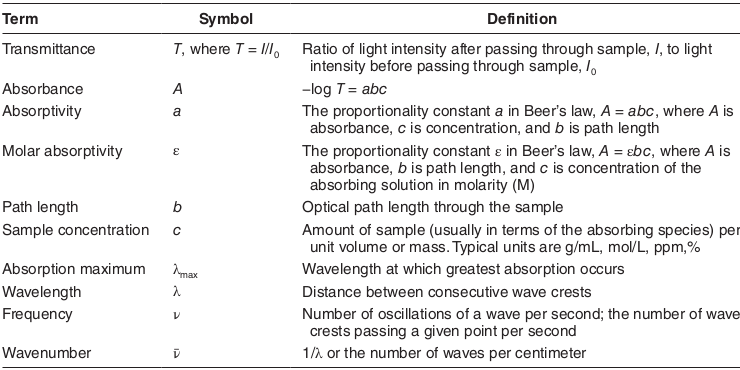
\includegraphics[width=0.9\textwidth]{2020-12-31_21-09.png}
\end{table}
\section{光学系统}
在光学分析光谱学中,测量样品对辐射的吸收或发射。用于测量辐射吸收或发射的仪器
必须提供有关吸收或发射的波长以及每个波长的强度(I)或吸收率(A)的信息。从光谱的
紫外到红外区域的光谱学研究仪器,其基本组成非常相似。目前,“光谱仪”将用于表示
用于光谱学的仪器。在讨论了组件之后,将为仪器定义更具体的术语。

用于分析光谱的仪器需要辐射源,波长选择设备(例如单色仪),对辐射范围透明的
样品架,用于检测辐射强度并将其转换为电信号的检测器,以及一些手段显示和处理
来自检测器的信号的过程。随后讨论的傅立叶变换(FT)光谱仪不需要波长选择设备。
如果要测量发射的辐射,则通过某种方式激发的样品就是辐射源。如果测量到光的吸收,
荧光,磷光或散射,则需要外部辐射源。这些组件的特定布置称为仪器的光学或光学配置
或光学布局。一个简单的单束吸收光谱仪的光学布局如图\ref{fig:2.17}所示。样品架和
波长选择器的放置可以颠倒;在UV/VIS吸收光谱法中,通常将样品架放置在波长选择器
之后,以使单色光落在样品上。对于原子吸收,红外和荧光光谱,通常将样品
放在波长选择器的前面。
\begin{figure}[htpb]
    \centering
    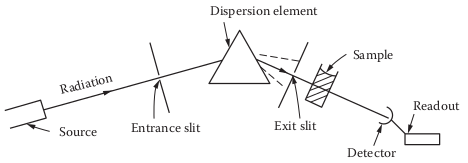
\includegraphics[width=0.75\textwidth]{2020-12-31_21-33.png}
    \caption{单束吸收光谱仪}
    \label{fig:2.17}
\end{figure}
\subsection{辐射源}
理想光谱辐射源应具备如下特征:
\begin{enumerate}
    \item 发射光必须涵盖所研究整个波长范围;
    \item 涵盖整个波长范围的辐射强度要足够高,可以避免来自检测器的信号放大;
    \item 光源在不同波长下,强度不应有明显变化;
    \item 光源强度不应随时间波动;
    \item 光源强度不应在短时间间隔内波动,这种波动称为“闪烁(flicker)”。
\end{enumerate}

辐射源的设计随其使用的波长范围而变化(例如,IR,UV,可见光),具体辐射源的详细
信息将在适当的仪器章节中进行讨论。大多数源的强度都会随电压的变化而呈指数变化,
因此在所有情况下,都需要向辐射源提供可靠,稳定的电源。电压调节器(也称为线路
调节器)可用来补偿输入电压的变化。如第2.6.5节所述,双光束光学配置也可用于补偿
光源稳定性的变化。

分析光谱中使用的辐射源有两种主要类型:连续体源和线源。连续谱源发出的辐射波长
范围很广,并且发射强度随波长的变化而缓慢变化。典型的连续体光源包括产生可见光
辐射(白光)的钨丝灯和高压氙弧灯,用于UV区的氘灯,用于UV区的高压汞或氙弧灯,
以及加热的固态陶瓷或光谱IR区域的加热线。连续谱源用于大多数分子吸收和荧光
光谱仪。相比之下,线源仅发射几个离散波长的光,强度是该波长的强函数。典型的线源
包括用于UV和可见光区域的中空阴极灯和无电放电灯,用于AAS和原子荧光光谱;用于UV
线的钠或汞蒸气灯(类似于现在在路灯中使用的灯)和可见光区域以及激光。激光是
高强度相干线光源;可提供在UV,可见光和IR区域具有发射线的激光。它们用作拉曼光谱
以及分子和原子荧光光谱中的来源。
\subsection{波长选择设备}
\subsubsection{滤波器}
选择电磁频谱某些部分的最简单、最便宜的方法是使用滤波器。有两种主要类型,吸收
滤波器和干涉滤波器。吸收滤光片可以像一块彩色玻璃一样简单。在第2.1节中,我们
讨论了蓝色玻璃如何透射可见光谱的蓝色波长,但吸收红色和黄色波长。这是用于
分离可见光谱的蓝色区域的吸收滤光器的示例。可以购买有色玻璃吸收滤光片,以隔离
各种范围的可见光。这些滤波器稳定,简单且便宜,因此非常适合用于便携式领域的
便携式光谱仪。最大的限制是与棱镜和光栅相比,透射的波长范围较宽。棱镜和光栅
也是用于从宽带多色光源中,选择较窄波长范围的设备。对于典型的吸收滤光片,透射
范围可能为50--300 nm。吸收滤光片仅限于光谱的可见光区域和X射线区域。

第二种类型的滤波器是干涉滤波器,由多层不同材料构成。该滤波器根据相长干涉原理
工作,以传输选定的波长范围。传输的波长由材料中心层的厚度和折射率控制。可以
构造干涉滤光片以透射光谱的IR,可见光和UV区域中的光。透射的波长范围比吸收滤光片
小得多,通常为1--10 nm,并且透射的光量通常比吸收滤光片高。
\subsubsection{单色器}
{\bf 单色器}由色散元件、入射狭缝和出射狭缝以及透镜和用于准直和聚焦辐射束的
反射镜组成。色散元件的功能是根据波长在空间中散射落在其上的辐射。两种最常见的
色散元件是棱镜和光栅。你可能已经很熟悉玻璃棱镜将白光分散为其组成
颜色的彩虹的功能。

入射狭缝允许来自光源的光落在色散元件上。分散的光落在单色器的出口狭缝上。出口
狭缝的功能是仅允许非常窄的光带穿过样品和检测器。实现此目的的一种方法是旋转
色散元件,以允许不同波长的色散光依次落在出口狭缝上。例如,白光源通过棱镜或光栅
,色散元件缓慢旋转,首先使紫色的光穿过出口狭缝,然后使蓝光等,一直到红光。
这样,单色器将来自光源的多色辐射分类为几乎单色的辐射,并离开出口狭缝。

\emph{棱镜}:棱镜用于分散IR、可见光和UV辐射。最常见的棱镜由用于紫外线区域的
石英,用于可见光和近红外(NIR)区域的硅酸盐玻璃,
\ce{NaCl}或\ce{KBr}用于IR区域。棱镜的形状像具有三角形横截面的条形。
$60^\circ–60^\circ–60^\circ$三角形(称为Cornu棱镜),如图\ref{fig:2.17}所示,
已被广泛使用,但也可以使用其他几何形状。穿过入口狭缝的多色光会聚在棱镜的一面上
,从而使入射光发生折射或弯曲。不同波长的光被折射到不同的程度,因此波长的空间
分离是可能的。棱镜材料的折射率随波长而变化。石英棱镜对短波辐射的折射率比
对长波辐射的折射率高;因此,短波辐射比长波辐射更易弯曲。如图\ref{fig:2.18}
所示,在光谱的可见区域中,通过这种棱镜时,红光的弯曲程度会小于蓝光。棱镜一直
以来是单色仪中最常用的分散设备,但已被衍射光栅或FT系统取代。
\begin{figure}[htpb]
    \centering
    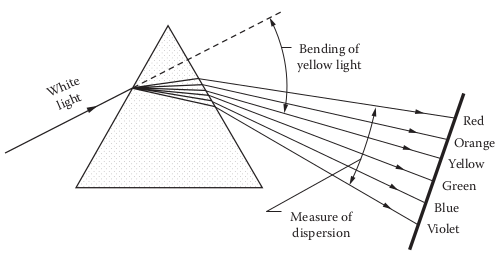
\includegraphics[width=0.65\textwidth]{2021-01-01_09-34.png}
    \caption{可见光通过棱镜色散}
    \label{fig:2.18}
\end{figure}

\emph{衍射光栅}:紫外线、可见光和IR辐射可以通过衍射光栅分散。衍射光栅由一系列
紧密间隔开的平行沟槽组成,这些沟槽被切成(或刻成)硬玻璃,金属或陶瓷表面
(图\ref{fig:2.19})。该表面可以是平坦的或凹入的,并且通常在直纹表面上涂覆
有反射涂层。用于紫外线和可见光区域的光栅将包含500至5000个凹槽/毫米,而用于
红外区域的光栅将具有50至200个凹槽/毫米。传统上,用金刚石工具对光栅中的凹槽
进行机械切割,这既费时又昂贵。这样的光栅被称为母版,并且用作从聚合物树脂浇铸
复制光栅的模具。复制光栅复制了原版中的凹槽,并涂有反射涂层,例如铝,以供使用。
大多数仪器使用复制光栅,因为它们比主光栅便宜得多。现在,大多数光栅都是通过
全息技术生产的。通过用光学平坦的光敏聚合物膜,涂覆光栅基板来制成光栅。
胶片暴露于激光束的干涉图样中,并且干涉图样被“燃烧”到胶片中。然后,使用化学或
离子蚀刻将干涉图案的凹槽蚀刻到基板中以制成主光栅,从而将凹槽成形为所需形状。
与机械刻划的主光栅相比,使用激光干涉图案形成凹槽可以以更低的成本获得更完美的
光栅。这些被称为全息光栅的光栅可以直接用于仪器中,也可以用作复制全息光栅
制造中的主光栅。全息光栅可以制成不同于传统平面或凹形的多种形状,并且根据应用,
凹槽的间距可以均匀或不均匀。典型的衍射光栅的尺寸在大约$25\times 25$到
$110\times 110$ mm之间变化。
\begin{figure}[htpb]
    \centering
    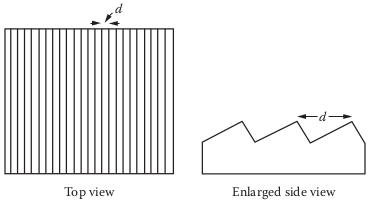
\includegraphics[width=0.65\textwidth]{2021-01-01_10-06.png}
    \caption{衍射光栅}
    \label{fig:2.19}
\end{figure}

光栅表面上的光分散是通过衍射发生的。反射光波之间的相长干涉,导致发生光衍射。
波的路径如图\ref{fig:2.20}所示。可以在相邻的凹槽上见到平行波。当发生
相长干涉或光衍射时
\begin{equation}
    n\lambda = d\left(\sin i \pm \sin\theta\right)
    \label{2.17}
\end{equation}
此处,$n$是光谱级次,其值可以取$1, 2, 3, \dots$整数;$\lambda$是入射光波长;
$d$是光栅相邻两刻痕间距离,称为光栅常数;$i$是光束入射角;$\theta$是波长
$\lambda$的光的散射角。
\begin{figure}[htpb]
    \centering
    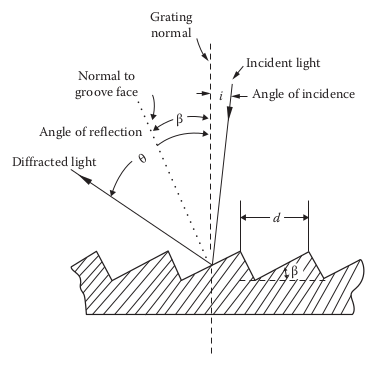
\includegraphics[width=0.65\textwidth]{2021-01-01_10-32.png}
    \caption{衍射光栅横截面:入射角$i$;衍射角$\theta$;光栅的闪耀角$\beta$;
    光栅间距$d$}
    \label{fig:2.20}
\end{figure}
入射角$i$和散射角$\theta$均从法线到光栅进行测量。$n$值一定,$\lambda$不同,
散射角不同。由于不同波长的光,以不同的角度衍射,发生光的分离。
\begin{figure}[htpb]
    \centering
    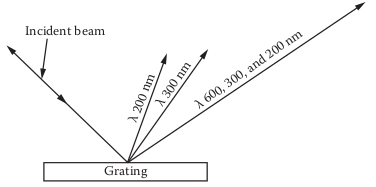
\includegraphics[width=0.65\textwidth]{2021-01-01_10-58.png}
    \caption{衍射角不但取决于波长,而且也取决于衍射级次$n$。波长为200、300
    300和600 nm的入射光,一阶($n=1$)不同的衍射角,但200 nm的三阶和300 nm的
二阶与600 nm的一阶重合}
\label{fig:2.21}
\end{figure}

光栅的一个问题是,几种不同波长的光可能以相同的色散角离开光栅。例如,假设
辐射束以角度$i$落在光栅上。对于给定的色散角$\theta$,根据公式\ref{2.17},
乘积$n\lambda$为常数。$n$和$\lambda$等于该常数的任何组合都将满足该方程式。
假设$\lambda = 600 nm$,$n = 1$给出了色散角$\theta$;那么,如果$\lambda=200 nm$
且$n = 3$,则角度也是$\theta$,依此类推。实际上,具有每个波长的辐射均以角度
$\theta$分散,并沿同一光路传播,如图\ref{fig:2.21}所示。以这种方式相关的光
的波长被称为衍射辐射的不同阶数。它们没有被光栅分开。色散后沿相同路径传播的
辐射的波长与数字$n$相关,该数字可以取任何整数的值。在高质量的光谱仪上,通过
使用小棱镜或滤光片系统作为与光栅结合的阶跃分选器,可以将不同阶分开
(图\ref{fig:2.22}和\ref{fig:2.23})。IR仪器通常将滤波器用作阶分类器。当光栅
旋转到不同的波长范围时,滤光片旋转以防止阶数重叠,并且只有一个波长到达检测器。
仪器公司Horiba Scientific(www.horiba.com)可以在Internet上找到有关衍射光栅和
光谱学的出色教程,方法是在主页上的搜索框中键入“光谱学教程”。
\begin{figure}[htpb]
    \centering
    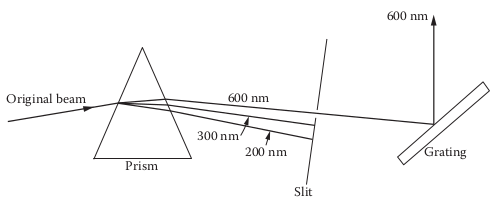
\includegraphics[width=0.75\textwidth]{2021-01-01_11-26.png}
    \caption{棱镜作为阶分类器}
    \label{fig:2.22}
\end{figure}
\begin{figure}[htpb]
    \centering
    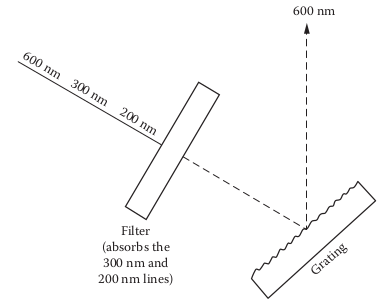
\includegraphics[width=0.65\textwidth]{2021-01-01_11-29.png}
    \caption{滤光片作为阶分类器}
    \label{fig:2.23}
\end{figure}
\subsubsection{分离两条不同波长所需的分辨率}
\emph{单色器波长精度}:在讨论系统分离两个波长的能力之前,评估系统的波长范围
非常重要。对于光谱的UV/VIS区域,可以通过扫描钬玻璃或钕镨玻璃,或市售的装有稳定
的高氯酸钬或高氯酸钕镨溶液的密封石英比色皿来完成。此类波长参考标准的一种来源
是Starna Cells,Inc.(www.starnacells.com)。如图\ref{fig:2.24}所示,这些化合物
会在整个UV/VIS区域产生一系列尖峰,应定期运行以确保从单色仪系统读取的波长准确。
可以使用类似类型的标准来检查远紫外和近红外区域的波长准确性。
\begin{figure}[htpb]
    \centering
    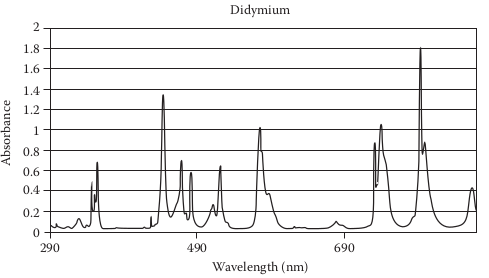
\includegraphics[width=0.85\textwidth]{2021-01-01_18-03.png}
    \caption{氧化钕镨UV/VIS波长参照光谱}
    \label{fig:2.24}
\end{figure}

\emph{单色器的分辨率}:分散辐射的能力称为分辨能力。替代名称包括色散功率和
分辨率。例如,为了观察599.9 nm的吸收带而不受600.1 nm的吸收带的干扰,我们必须
能够分辨或分离这两个带。

单色器的分辨能力$R$等于$\lambda /\delta\lambda$,其中$\lambda$是要分辨的两条线
的波长的平均值,而$\delta \lambda$是这两条线之间的波长差。在本示例中,
所需的分辨率为
\begin{equation}
    R=\frac{\lambda}{\delta\lambda}
    \label{2.18}
\end{equation}
\[
    R=\frac{\text{Average of 599.9 and 600.1}}
    {\text{Absolute difference between 599.9 and 600.1}}
    =\frac{600}{0.2}=3000
\]

\emph{棱镜的分辨率}:棱镜的分辨率$R$为
\begin{equation}
    R = t\frac{d\eta}{d\lambda}
    \label{2.19}
\end{equation}
此处,$t$是棱镜底部厚度;$d\eta/d\lambda$是棱镜材料的色散能力(或折射率)
$\eta$随波长的变化率。对于波长$\lambda_1$和$\lambda_2$的两个光束,棱镜的
折射率不相同。如果为常数,则不会发生分辨。棱镜的分辨能力随棱镜的厚度而增加。
通过选择棱镜材料,使$d\eta/d\lambda$最大,可以使给定波长区域的分辨率最大化。
例如,玻璃棱镜比石英棱镜更好的散射可见光。为了获得最大的色散,棱镜在接近于
不再透明的波长处最有效。
For maximum dispersion, a prism is most effective at wavelengths close to
the wavelengths at which it ceases to be transparent.
在更长的波长处,分辨率降低。

\emph{光栅分辨率}:光栅分辨率由下式给出
\begin{equation}
    R = nN
    \label{2.20}
\end{equation}
此处,$n$是级次(阶数);$N$是入口狭缝发出的光,照亮的光栅凹槽总数。因此,较长
的光栅,较小的凹槽间距,以及高阶数($n>1$)的使用会提高分辨率。假设我们可以
获得一个500/cm的光栅。一阶将589.5 nm和589.0 nm处的钠D线分开,需要多长光栅?
从式\ref{2.18}可知,所需分辨率$R$如下
\[
    R = \frac{589.25}{0.5}=1178.5
\]
光栅分辨率至少需要1179(四位有效数字)。但(光栅)$R=nN$,即$1179=nN$。由于
我们规定为一阶,$n=1$;因此,$N$所需凹槽总数,是1179。光栅每厘米包含500线。
于是,解得(1179/500),即2.358 cm。

另一种问法,每厘米多少凹槽,才能在3.00 cm内分辨出相同的钠D线(假设整个光栅都被
照亮)?需要1179的分辨率,对于一阶来说,总计需要凹槽数量为$nN=N=1179$,所以
\[
    N/cm = 1179/3.00 cm = 393 \text{lines/cm}
\]
不可能刻蚀出分数的凹槽,$N$必定为整数,计算结果取最接近整数。

实际中,通常测试苯蒸气来评估紫外线中的光栅单色器系统的分辨率,这会产生许多
紧密而尖锐的吸收线。市场上有售苯蒸气的密封石英池可用于评估。通常在几个带宽下
进行评估,如图\ref{fig:2.25}所示。
\begin{figure}[htpb]
    \centering
    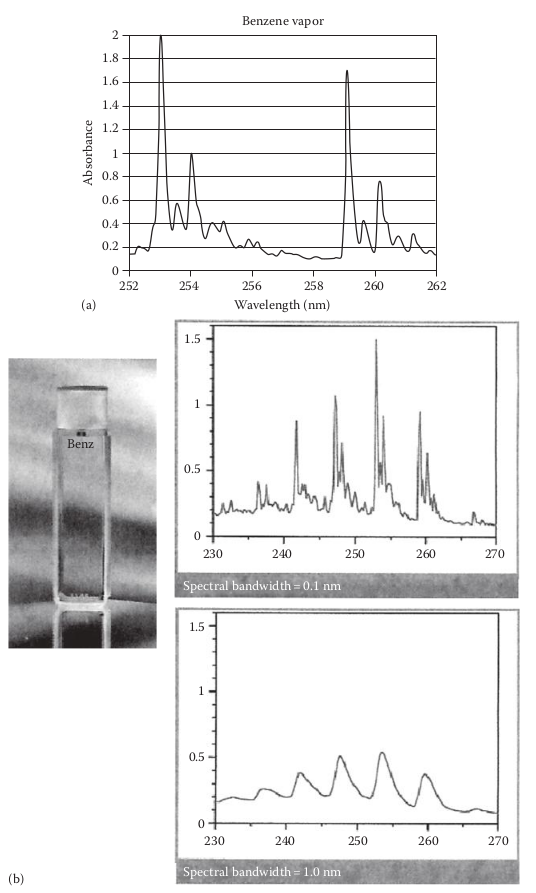
\includegraphics[width=0.85\textwidth]{2021-01-01_22-29.png}
    \caption{(a)苯蒸气光谱;(b)两种不同带宽下苯蒸气光谱}
    \label{fig:2.25}
\end{figure}

\emph{光栅单色器的色散}:衡量单色器分辨率的能力,就是看相邻波长的光是否能分开。
分辨率与倒数色散(或线性倒数)$D^{-1}$有关:
\begin{equation}
    D^{-1}=\frac{d\lambda}{dy}
    \label{2.21}
\end{equation}
线性色散的倒数等于波长的变化$d\lambda$与相应$y$的变化的比值,即,沿色散轴分割
波长的距离。$D^{-1}$的单位通常为nm/mm。$D^{-1}$作用在于,离开单色器的光的光谱
带宽(SBW)或光谱带通与$D^{-1}$和狭缝宽度直接相关:
\[
    \text{SBW}=sD^{-1}
\]
此处,$s$是单色器狭缝宽度。SBW表示离开单色器的光的75\%的波长范围的宽度。使用
光栅作为色散设备的单色器,线性色散倒数为
\begin{equation}
    D^{-1}=\frac{d}{nF}
    \label{2.23}
\end{equation}
$d$是光栅两个凹槽间距;$n$是衍射阶;$F$是单色器系统的焦距。因此,基于光栅的系统
相互色散在波长方面基本恒定。UV区域的SBW可以通过使用匹配的己烷中的溶液来确定。
在268.7 nm和267.0 nm处测量吸光度。计算吸光度比($A_{268.7}/A_{267.0}$),并与
SBW直接相关,如表\ref{tab:2.11}和图\ref{fig:2.26}所示。基于棱镜的单色器的色散
是更复杂的计算。
\begin{table}[htbp]
    \centering
    \caption{波长比率的带宽}
    \label{tab:2.11}
    \begin{tabular}{lccccr}
        \hline
        Ratio & 2.5 & 2.1 & 1.6 & 1.4 & 1.0 \\
        SWB   & 0.5 & 1.0 & 1.5 & 2.0 & 3.0 \\
        \hline
    \end{tabular}
\end{table}
\begin{figure}[htpb]
    \centering
    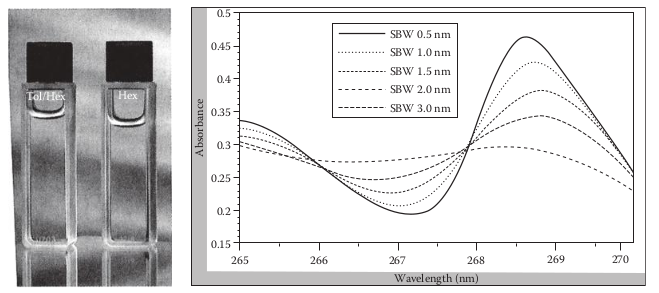
\includegraphics[width=0.85\textwidth]{2021-01-02_11-09.png}
    \caption{光谱带宽的测量(0.02\%甲苯的正己烷溶液)}
    \label{fig:2.26}
\end{figure}

\emph{Echelle单色器}:从图\ref{fig:2.19}和\ref{fig:2.20}可以看到,光栅表面上
显示的切口不是对称的$V$型。每个切口都有一个短面和一个长面。这种光栅称为闪耀
光栅(blazed grating)。如图\ref{fig:2.20}所示,常规的闪耀衍射光栅使用的凹槽的
长面,通常针对一阶衍射优化闪耀角$\beta$的切割角度。可以裁定具有更高闪耀角的
光栅,并可以使用凹槽的短面进行衍射;这种刮擦称为阶梯光栅。阶梯光栅的色散角
$\beta$比传统光栅高得多。echelle系统通过增加$\theta$角和使用更高阶(较大$n$
值)来改善色散。结果是,与相同焦距的常规光栅单色器相比,分辨率提高10倍。由于
衍射的多个高阶,因此有必要使用第二个分散元素对重叠的阶进行排序。第二个色散元件
,成为交叉色散器,用来对与光栅成直角的光进行分类,从而获得2D光谱。ICP发射光谱
(ICP-OES)的echelle光学布局如图\ref{fig:2.27}所示,图\ref{fig:2.28}显示2D
输出的示例,波长在$y$轴上绘制,衍射级在$x$轴。
\begin{figure}[htpb]
    \centering
    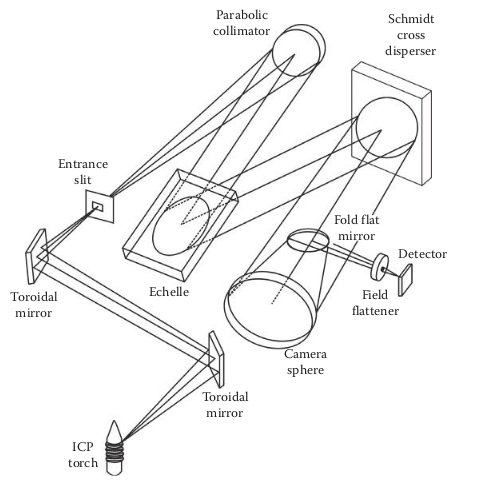
\includegraphics[width=0.75\textwidth]{2021-01-02_12-56.png}
    \caption{echelle光学布局}
    \label{fig:2.27}
\end{figure}
\begin{figure}[htpb]
    \centering
    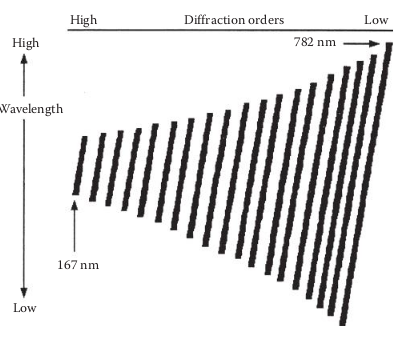
\includegraphics[width=0.75\textwidth]{2021-01-02_12-57.png}
    \caption{echelle光谱产生的色散2D阵列}
    \label{fig:2.28}
\end{figure}

\subsection{狭缝}
狭缝系统(图\ref{fig:2.17})用于从波长选择器分散光束之前和之后的光束中选择辐射
。狭缝的钳口由金属制成,通常形状像两个刀刃。它们可以彼此相对移动以根据需要改变
狭缝的机械宽度。为简单起见,图\ref{fig:2.17}并未显示单色器中用于根据需要
聚焦和准直光的透镜或反射镜系统。

入口狭缝允许来自光源的光束通过。来自光源的辐射聚焦在入口狭缝上。杂散辐射被排除
在外。通过入口狭缝后,辐射被准直成平行光束,该光束落在棱镜或整个光栅的一侧
并完全照亮。棱镜或光栅根据波长将光分散到不同的方向。在为色散设备选择的设置下,
将一个波长重新聚焦到出口狭缝上。其他波长的光也会聚焦,但不会聚焦到出口狭缝上。
发出的光线被重定向并聚焦到检测器上以进行强度测量。

透镜或前视镜用于聚焦和准直光。在红外中,前视镜总是比镜头更有效,并且不吸收辐射
。它们也很容易被刮擦,因为反射面在前部并且不受玻璃保护,就像常规镜子一样。
不使用背面镜,因为覆盖材料(例如玻璃)可能吸收辐射。图\ref{fig:2.29}显示了一种
类型的单色仪系统,该系统使用反射镜进行聚焦,准直,并使用光栅进行分散,
并显示了入口和出口狭缝。
\begin{figure}[htpb]
    \centering
    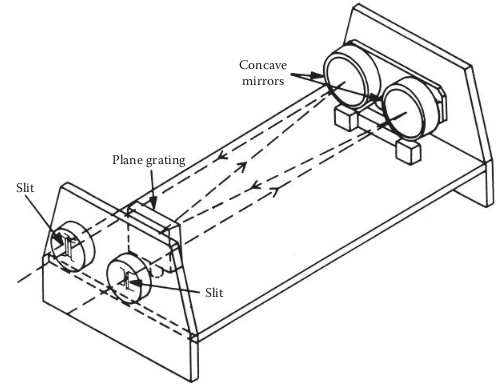
\includegraphics[width=0.85\textwidth]{2021-01-02_13-15.png}
    \caption{光栅单色器和狭缝}
    \label{fig:2.29}
\end{figure}

缝隙的钳口之间的物理距离称为机械缝隙宽度。以前装有千分尺的仪器,以便可以直接
读取机械狭缝的宽度;现代计算机控制的仪器通过控制运行狭缝机构的步进电机的软件
来设置和读取狭缝宽度。在紫外吸收光谱中,机械狭缝宽度约为0.3--4 $\mu m$。在红外
光谱中,色散仪器的缝隙宽度通常在0.1到2.0 mm之间。FTIR光谱仪中没有狭缝。

穿过出口狭缝的辐射的波长范围称为光谱带通或光谱带宽。如前所述,该带通可以通过
使用甲苯在己烷中的吸收光谱来测量。也可以通过将很窄宽度的发射线穿过狭缝到达
检测器来进行测量。通过旋转色散元件,我们可以记录发生响应的波长范围。校正发射线
的实际宽度后,我们可以计算光谱带通。例如,要测量用作AAS的单色仪系统的光谱带通,
我们可以使用镉空心阴极灯,它从镉产生非常窄的原子发射线。这些线之一出现在
228.8 nm。我们移动分散设备并在检测器上监视信号。镉的发射线在228.2至229.4 nm的
所有波长下发出信号。这意味着镉发射线在1.2 nm宽的波长范围内到达检测器。因此,
1.2 nm是此单色仪系统的光谱带通。在此示例中,未对228.8 nm镉线的实际宽度
进行校正,在这种情况下可以忽略不计。在上述实验中测量的信号具有高斯峰形状。
此类测量中的SBW通常定义为最大峰值高度的一半处的信号峰值宽度,称为半峰全宽
(FWHM)。光谱带通通常为0.3--4 nm。请注意,SBW比物理缝隙宽度(nm对$\mu$m)
小三个数量级。

如果机械狭缝的宽度变宽,则谱带通将同时增加,反之亦然。光谱带通是光谱仪中
影响分辨率的组件之一,如图\ref{fig:2.25}所示。例如,利用所描述的机械狭缝设置,
将不可能分辨出从228.8 nm \ce{Cd}线到229.0 nm处的发射线,因为两者都将穿过狭缝。
在实践中,缝隙应尽可能地窄以确保最佳分辨率。但是,它们必须足够宽,以允许检测器
测量足够的光。狭缝宽度的最终选择由分析师根据手头的特定样品确定。一个好的经验
法则是在不损害检测器功能或检测指定量分析物的能力的情况下,使缝隙尽可能窄。

通过旋转棱镜或光栅(或通过使出口狭缝横穿单色仪发出的光束),可以改变通过出口
狭缝的波长范围。通过将色散元件从一个极端连续旋转到另一个极端,
可以扫描整个光谱。
\subsection{检测器}
检测器用于测量落在其上的辐射强度。通常,它是通过将辐射能转换为电信号来实现的。
产生的能量通常很少,必须放大。来自检测器的信号必须稳定,并代表落在其上的
辐射强度。如果信号放大太多,它将变得不稳定,噪音多。信号中的随机变化程度称为
噪声级别。放大来自检测器的信号会增加其响应。在实践中,可以增加响应,直到信号
的噪声级别变得太大为止;否则,可能会增加响应。在这一点上,放大率降低,
直到噪声级别可以接受为止。

存在许多不同类型的光子检测器,包括光电倍增管、硅光电二极管、光伏电池以及
一类称为电荷转移设备的多通道检测器。电荷转移检测器包括光电二极管阵列、
电荷耦合器件(CCD)和电荷注入器件(CID)。这些检测器用于
原子/分子光谱学的UV/VIS和IR区域。

除光子探测器外,还有几个重要的探测器可以测量热量。这些热探测器在光子能量非常低
的IR区域特别有用。这些检测器将在以下各章中详细讨论特定技术,例如,IR检测器,
光电倍增管检测器和光电二极管、CCD和CID。
\subsection{单光束和双光束}
\begin{figure}[htpb]
    \centering
    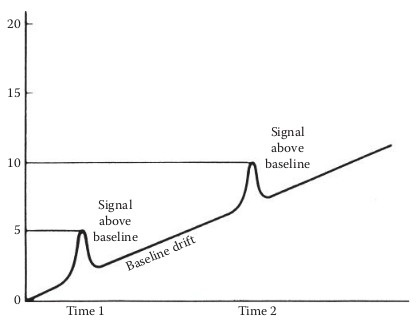
\includegraphics[width=0.85\textwidth]{2021-01-02_13-38.png}
    \caption{光谱测量中由于基线漂移导致的误差}
    \label{fig:2.30}
\end{figure}
如图\ref{fig:2.17}所示,单光束光学器件用于所有光谱发射方法。在发射过程中,将
样品放在图\ref{fig:2.17}中的源所在位置。在光谱吸收研究中,必须测量穿过样品
之前和之后的辐射强度。当使用单光束光学器件时,在进行测量时光源强度的任何变化
都可能导致分析误差。平均信号随时间的缓慢变化称为漂移,如图\ref{fig:2.30}所示。
漂移会导致所得结果直接错误。信号在时间0被设置为零,没有分析物存在。随着时间
朝着时间1增加,不存在分析物的信号(称为基线信号)由于漂移而增加。在时间1,由于
存在分析物(峰在基线上方显示),样品被测量并给出增加的信号。在时间1处的总信号
(样本加基线)为5个单位。基线继续向上漂移,在时间2,再次测量样品。从图中可以
看出,样品在基线以上的峰高与时间1的峰高相同,但是总信号(峰加基线)现在为10个
单位。如果不考虑基线漂移,分析人员将得出结论,时间2的样品分析物是时间1的两倍,
这是直接误差。

漂移的来源很多。辐射源强度可能由于线性电压的变化,源在最近打开后预热或源随时间
而改变。单色器可能会由于振动或加热和冷却而移动位置,从而导致膨胀和收缩。检测器
的线性电压可能会发生变化,或者检测器可能会随着时间而变差并导致响应发生变化。
与校准中使用的标准相比,由漂移引起的误差会导致发射信号或吸收信号的测量误差。
通过不断检查光强度或使用分析过程中以频繁间隔测量的标准溶液,可以减少此问题。
单光束光学器件尤其容易受到漂移引起的误差的影响。但是,通过使用双光束系统
可以大大减少与漂移相关的问题。

\begin{figure}[htpb]
    \centering
    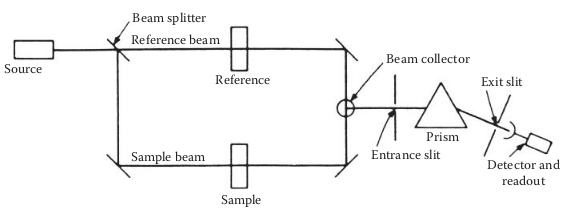
\includegraphics[width=0.85\textwidth]{2021-01-02_15-11.png}
    \caption{双光路系统}
    \label{fig:2.31}
\end{figure}

双光束系统广泛用于光谱吸收研究。系统的各个组件与单光束系统具有相同的功能,
但有一个非常重要的区别。使用分束器将来自源的辐射分成强度近似相等的两束光束,
如图\ref{fig:2.31}所示。一束称为参考束;穿过样品的第二束称为样品束。然后将两个
光束重新组合,并通过单色器和狭缝系统到达检测器。图\ref{fig:2.31}对此进行示意性
说明。在此示意图中,参考光束中有一个单元与用于保存样品的单元相同。例如,参比池
可以是空的,也可以包含用于稀释样品的溶剂。样品后显示单色器的这种特殊安排是
分散IR双光束分光光度计的典型特征。双光束系统的光学布局有许多商业上的变化。

\begin{figure}[htpb]
    \centering
    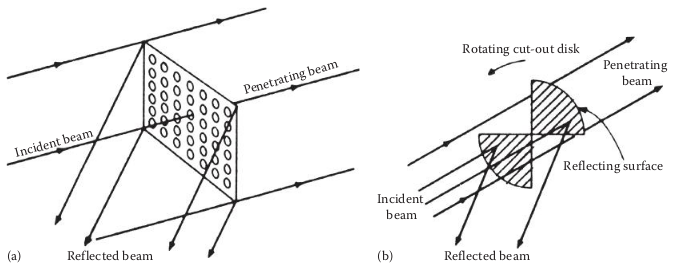
\includegraphics[width=0.85\textwidth]{2021-01-02_15-13.png}
    \caption{(a)板式分束器;(b)旋转分束器}
    \label{fig:2.32}
\end{figure}
\begin{figure}[htpb]
    \centering
    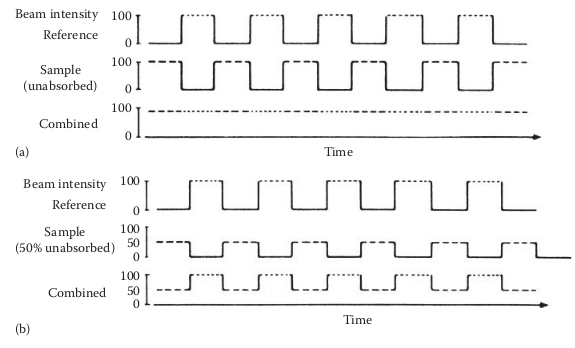
\includegraphics[width=0.85\textwidth]{2021-01-02_15-15.png}
    \caption{经过旋转分束器达到检测器的辐射强度:(a)没有吸收;(b)吸收50\%}
    \label{fig:2.33}
\end{figure}

如图\ref{fig:2.32}(a)所示,分束器可以是一个简单的镜板,在其中钻有许多孔。光被
镜板反射并向下穿过样品光束路径。相等的一部分光穿过板上的孔并形成参考光束。
另一个方便的分束器是去除相对象限的盘(图\ref{fig:2.32}(b))。圆盘在辐射束的前面
旋转,镜面将光反射到样品路径中。丢失象限允许辐射沿参考路径通过。每束光束都是
断续的,并以交变信号的形式到达检测器。当样品没有吸收任何辐射时,两个光束相等,
重新结合并形成稳定的光束。但是,当辐射被样品吸收时,两个光束不相等,并且交替
信号到达检测器。如图\ref{fig:2.33}所示。

使用双光束系统,我们可以测量参考光束强度与样本光束强度的比率。因为使用了比率,
所以在测量过程中来自源的辐射强度的任何变化都不会引起分析误差。这一优势彻底
改变了吸收光谱。如果信号中存在漂移,则它会同样影响样本和参考光束。除非漂移非常
大,否则重组光束将继续提供准确的信号信息,在这种情况下,校正不会完成。使用
双光束系统进行的吸收测量实际上与漂移无关,因此更准确。
\subsection{傅立叶变换光谱仪}
前述的色散光谱系统将光分成其分量波长,并将其传播到光谱中。在这些系统中,可以
沿着波长与位置成比例的路径在每个点处测量强度。可以通过缓慢移动光栅来确定光谱中
每个点周围狭窄区域的强度,以使分散光谱的每个区域都通过单个固定检测器。或者,
系统可以使用连续的检测器阵列同时测量所有波长区域。后一种方法可在更少的时间内
获取更多信息。它可以通过使用一维光电二极管阵列或2D CCD在UV/VIS区域中实现,这与
现代数码相机中的类似。

能量较低的红外波长的检测器无法轻易小型化,因此色散红外采用慢扫描方法工作。为了
使用扫描仪器获得高波长分辨率,需要将到达检测器的波长区域限制在非常窄的窗口内。
反过来,这需要缓慢扫描光谱以达到所需的灵敏度。

FT光谱仪采用的光谱采集方法与色散系统中使用的光谱采集方法截然不同。理想的是同时
测量所有波长的光,其方式应允许强度与波长曲线(即光谱)的重建。如果波长信息
以明确定义的方式编码,例如通过使用干涉仪对光强度进行调制,则数学方法可以将信息
解释和呈现为从色散仪器获得的相同类型的光谱。在没有分散设备的情况下执行此操作
的仪器称为多路复用仪器。如果同时收集所有感兴趣的波长而不分散,则这些波长及其
相应的强度将重叠。必须对产生的重叠信息进行分类以绘制频谱。排序或“解卷积”变化
频率(或波长)的重叠信号的常用方法是一种称为傅立叶分析的数学程序。此处介绍的
示例是IR光谱学,它是仪器分析化学中的第一个应用程序,但是该原理还与其他技术结合
使用,在这些技术中,分析数据显示为响应随频率变化的频谱,例如NMR和离子回旋
共振MS。

傅里叶分析允许将任何连续曲线(例如,强度峰和谷的复杂光谱作为波长或频率的函数)
表示为随时间变化的正弦或余弦波之和。相反,如果可以将这些正弦波和余弦波的等效值
作为数据来获取,则可以将其进行傅立叶变换成频谱曲线。这就要求以数字形式进行数据
采集,强大的计算能力和高效的软件算法,而这些功能现在已经可以在当前的
个人计算机,笔记本电脑和手持设备的级别上轻松获得。例如,采用这种方法的计算机
化仪器称为FT光谱仪-FTIR,FTNMR和傅里叶变换质谱(FTMS)仪器。

FT光谱仪使用的干涉仪在设计上类似于图\ref{fig:2.34}所示的迈克尔逊干涉仪。为了
简化讨论,我们首先考虑产生波长为$\lambda$的单色辐射的光源。源辐射射到分束器上,
分束器将一半的光透射到固定镜,其余的反射到移动镜。可以对移动镜进行编程,使其
以精确控制的恒定速度沿光束路径移动。光束从镜子反射回分束器。每束光线的一半直接
穿过样品架到达检测器。其他两半沿源的方向向后移动,无需进一步考虑。如果固定镜和
移动镜与分束器的距离完全相等,则两个半光束将同相合并。组合波的振幅将是每个半波
的两倍,并且检测器信号将达到最大。如果移动镜随后移动等于$\lambda / 4$的距离,
则两个半光束将异相合并180$^\circ$(即$\lambda/ 2$)。光束产生相消干涉,检测器
未记录任何信号。对于反射镜之间的路径差的所有其他值,会发生部分相消干涉。当移动
镜以恒定速度移动时,到达检测器的信号会通过这种相长和相消干涉的重复模式有规律地
循环。当路径差$\delta$是$\lambda$的整数倍时,它最大化;当$\delta$是$\lambda$的
半整数倍时,它变为零。在FTIR中,$\delta$称为延迟。对于单色光,信号(功率,
强度)与$\delta$的关系图称为干涉图,其形式为简单的纯余弦曲线:
\begin{equation}
    P(\delta)=B(\bar{u})\cos(2\pi\delta\bar{u})
    \label{2.24}
\end{equation}
$P(\delta)$是达到检测器喜好的幅度;$B(\bar{u})$是一个与频率相关的常数,说明仪器
的变量,例如检测器响应,分束器投射或反射的光量以及光源强度。
波数$\bar{u}$等于$1/\lambda$。干涉图是到达检测器的干扰信号的记录。它实际上是
一个“时域”频谱。它记录检测器响应随时间变化的方式。如果样品吸收特定频率的光,
则该频率的幅度会发生变化。对于连续光源(在感兴趣区域内所有波长的输出具有连续
可变输出的光源),干涉图是一条复杂曲线,可以表示为无穷余弦波和反射光吸收的
不同幅度的总和通过样本。尽管很复杂,但是如果在足够数量的点处对干涉图进行采样,
则使用快速傅里叶变换(FFT)的现代计算机可以处理干涉图并识别足够的余弦波,从而
可以将数据解卷积为强度的IR光谱图与波长的关系。
\begin{figure}[htpb]
    \centering
    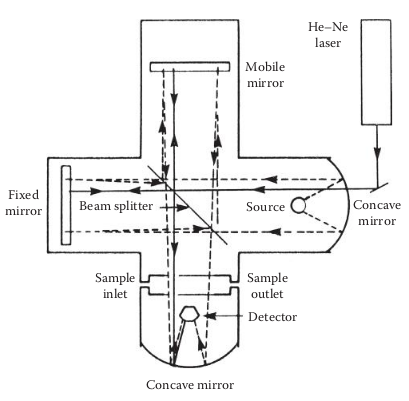
\includegraphics[width=0.85\textwidth]{2021-01-02_16-43.png}
    \caption{FTIR光谱仪}
    \label{fig:2.34}
\end{figure}
\subsubsection{傅立叶系统的优点}
与分散系统相比,FT光谱仪产生更好的信噪比。这是由几个因素造成的。 FT仪器的光学
元件较少且没有狭缝,因此到达检测器的辐射强度比色散仪器高得多。信号的增加会增加
信噪比。这称为吞吐量优势或雅奎诺特优势。同时测量所有可用波长,因此大大减少了
收集所有数据以形成光谱所需的时间。整个红外光谱可以在不到1秒的时间内收集到。这
使得实用的频谱测量的数百次重复的收集和信号平均化成为可能。信号平均对S/N的理论
改进与平均频谱数$(n)^{1/2}$的平方根成正比。这种优势称为多路复用或Fellgett优势。

FT光谱仪具有很高的波长重现性。在FTIR光谱仪中,移动镜在移动过程中的位置通过
光学系统使用来自可见范围激光器的高度单色光的平行干涉测量法以极高的精度连续进行
校准,如图\ref{fig:2.34}所示。在干涉图进行傅立叶变换之后,这种精确的位置测量
结果可以转换为准确且可重现的分析波长测量结果。这种精确的位置测量可以精确地
添加多个光谱,从而获得多重优势。

应该注意的是,FT光谱仪是单光束仪器。背景必须与样品光谱分开收集。这两个光谱的
比率导致背景校正的光谱,类似于从双光束仪器获得的光谱。尽管不能同时采集样品和
背景光谱,但由于可以快速采集和快速处理光谱,因此可以定期采集背景光谱,以避免
单光束色散仪遇到的问题。
\section{光谱技术和仪器命名}
光谱学和光谱仪器已经发展了许多年。毫无疑问,所使用的术语也已经发展并且实际上
正在不断发展。科学术语通常是由专业组织定义的,有时这些组织在定义上不一致,从而
导致使用同一术语来表示不同的含义。科学家(和学生)必须及时了解术语的含义以进行
有效的交流,但还必须了解术语的较旧用法才能理解文献。光谱学一词是指研究电磁辐射
与物质的相互作用。术语“光谱法”用于定量测量一个或多个电磁辐射波长的强度。分光
光度法是保留用于吸收测量的术语,其中必须在双光束系统中同时测量或在单光束系统中
依次测量两种强度(样品和参考)的比率。该术语逐渐被光谱学取代;例如,atomic
absorption spectrometry比atomic absoption spectrophotometry更普遍。

用于仪器的术语通常区分如何选择波长或使用的检测器类型。光谱仪是一种由棱镜或光栅
色散装置,狭缝和光电检测器组成的仪器,用于测量透射率或吸收率。但是,术语
“光谱仪”现在也适用于非分散且没有狭缝的基于IR干涉仪的FT系统。分光光度计是指
双光束光谱仪;但是,该术语现在同时用于吸收测量的单光束和双光束色散光谱仪。
光度计是一种光谱仪,它使用滤光片来选择波长而不是色散装置。光谱仪是一种具有
分散装置的仪器,该仪器具有较大的孔径而不是微小的出口狭缝,并且使用照相胶片进行
检测(现已淘汰)或使用固态成像检测器。
\newpage
\section{实验练习}
\begin{exercise}\label{exer:1.1}
UV/VIS光谱仪、样品池等。
\begin{enumerate}[a.]
\item 制备标准溶液:(1)0.1 g/L \ce{KMnO4}水溶液;(2)1.0 g/L \ce{K2Cr2O7}水溶液
    ;(3)用水稀释50\%的红墨水溶液。
\item 在350--700 nm范围内检测三种溶液的最大吸收波长。
\item 计算三种溶液最大吸收波长处的透射率$I/I_0$。
\end{enumerate}
\end{exercise}
\begin{exercise}
\begin{enumerate}[a.]
\item 练习\ref{exer:1.1}(a)中选择一种标准溶液(标记为A),测试最大吸收处的透射
    率。取50 mL至100 mL容量瓶中,去离子水定容(标记为B)。测量和记录溶液B的透射
    率。取50 mL溶液B,定容于100 mL容量瓶中(标记为C),测量和记录溶液C的透射率
    。如此类推,溶液D、E和F。
\item 以A到F的数据,拟合、绘制透射率-浓度曲线。
\item 计算每种溶液的吸光度,并拟合、绘制吸光度-浓度曲线。
\item 计算未知浓度溶液,使用那张图更合适一些?为什么?
\end{enumerate}
\end{exercise}
\begin{exercise}
\begin{enumerate}[a.]
\item 取练习\ref{exer:1.1}配置\ce{KMnO4}溶液10.0 mL,并加入该练习配置的
    \ce{K2Cr2O7}溶液10.0 mL,混合后,测量吸收。
\item 取10.0 mL\ce{K2Cr2O7}溶液加到10.0 mL去离子水中,并测量吸收。
\item 取10.0 mL\ce{KMnO4}溶液加到10.0 mL去离子水中,并测量吸收。使用每种化合物
    最大吸收波长,回答下面问题。与包含单一化合物的溶液相比,包含两种化合物的
    溶液最大吸收波长处的吸光度有没有变化?单一溶液吸收的光总量等于混合物吸收
    光量之和吗?吸光度的这种变化(如果有的话)会导致误差吗?误差是正还是负?
    如果必须测量\ce{KMnO4}和\ce{K2Cr2O7}混合物,你能想到纠正此误差的方法吗?
\end{enumerate}
\end{exercise}
\begin{exercise}
在其最大吸收波长下,测量新鲜制备的\ce{KMnO4}水溶液的吸收率。溶液的浓度应使
吸光度约为0.6--0.8。将溶液放入容量瓶中,然后将溶液直接从容量瓶中倒入样品架中
进行首次测量。现在,将溶液从烧瓶中倒入烧杯或宽口广口瓶中(您要使表面积最大化)
。让溶液在大气中暴露5分钟,然后再次测量溶液的吸光度。每隔5分钟重复一次测量。
(如果看不到变化,则将样品盖好并摇匀,然后解开盖,使其在空气中静置。)相对于
暴露在空气中的时间绘制测得的吸光度。这种变化是由\ce{KMnO4}的化学不稳定(它与
空气反应)引起的。如果将其用作校准的标准解决方案,则此更改将导致错误。许多标准
解决方案或多或少都会受到此类错误的影响,因此必须采取预防措施来防止和避免这种
麻烦。建议使用两种方法来避免\ce{KMnO4}出现此问题。
\end{exercise}
\newpage
\begin{problemset}
\item 分子吸收频率为$3.00\times 10^{14} Hz$的辐射,两个能级差是多少?
\item 波长为$500.0 nm$的辐射,频率是多少?
\item 描述原子吸收UV辐射所发生的跃迁。
\item 按波长递增的顺序排列:IR, radiowaves, X-rays, UV, visible light。
\item 对于给定的跃迁,原子或分子的吸收程度是否取决于基态或激发态的数量?为什么?
\item 对于给定的跃迁,云子或分子的发射程度是否取决于基态或激发态的数量?为什么?
\item 简要描述大多数分子中发生的三种跃迁类型,和跃迁中所涉及的辐射类型。
\item 简述Beer-Lambert-Bouguer定律的数学公式,并解释等式每个符合的含义。
\item (a)定义透射率和吸光度;(b)浓度与(1)透射率(2)吸光度之间有什么关系?
\item 使用图2.16,通过将线延长到覆盖浓度差异的10倍,来计算通过标记为B的较低点
    绘制切线的斜率。通过找到曲线上部分的斜率等于刚计算出的斜率,来确认相对误差
    为1\%(\% RE)的B--B所示范围是正确的。重复计算C点并确认C--C范围。
\item 通过在$510 nm$和$1.00 cm$光路下测量反应\ce{Fe^2+}与1,10-菲啰啉红色络合物
    溶液的透射率,在用于铁含量测定的外标校准中获得以下数据
    \begin{table}[htbp]
        \centering
        \begin{tabular}{llll}
            \hline
            铁浓度(ppm)&透射率(\% T)&铁浓度(ppm)&透射率(\% T)\\
            \hline
            0.20 & 90.0 & 3.00 & 26.3 \\
            0.40 & 82.5 & 4.00 & 17.0 \\
            0.60 & 76.0 & 5.00 & 10.9 \\
            0.80 & 69.5 & 6.00 & 7.0 \\
            2.00 & 41.0 & 7.00 & 4.5 \\
            \hline
        \end{tabular}
    \end{table}

    (a)计算每种溶液的吸光度$A$,并绘制吸光度-铁浓度曲线(你可以使用电子表格
    程序)。
    系统在整个浓度范围内是否符合Beer定律?(b)计算平均摩尔吸光系数;(c)绘制
    透射率(100--\% T)相对于浓度对数曲线图(Ringbom法),(1)在此范围内最佳浓度
    范围和最大准确度是多少?(每1\%透射率误差的\%RE)(2)在什么浓度范围内,每
    1\%透射率误差的相对分析误差不超过5\%?
\item 下表是标准曲线法测定铜(\ce{Cu(NH3)4^2+})数据
    \begin{table}[htbp]
        \centering
        \begin{tabular}{llll}
            \hline
            铜浓度(ppm)&透射率(\% T)&铜浓度(ppm)&透射率(\% T)\\
            \hline
            0.020 & 96.0 & 0.800 & 27.8 \\
            0.050 & 90.6 & 1.00 & 23.2 \\
            0.080 & 84.7 & 1.40 & 17.2 \\
            0.100 & 81.4 & 2.00 & 12.9 \\
            0.200 & 66.7 & 3.00 & 9.7 \\
            0.400 & 47.3 & 4.00 & 8.1 \\
            0.600 & 35.8 &  &  \\
            \hline
        \end{tabular}
    \end{table}

    计算每一溶液的吸光度,绘制吸光度--铜浓度曲线。在这些条件下,进行测量的系统
    在整个浓度范围内是否符合Beer定律?是否有小量的或大量的定律偏离?提出任何
    可能的偏差产生原因。
\item 将$0.200 g$铜溶于硝酸中,加入过量的氨生成\ce{Cu(NH3)4^2+},定容至1 L。
    分别取该溶液10.0, 8.0, 5.0, 4.0, 3.0, 2.0和1.0 mL,并定容于10.0 mL。对应的
    吸光度分别为0.500, 0.400, 0.250, 0.200, 0.150, 0.100和0.050。通过形成
    \ce{Cu(NH3)4^2+}络合物并测量吸光度来分析一系列样品的浓度。吸光度为(a)
    0.450 (b) 0.300 (c) 0.200 对应铜的浓度是多少?如果通过分别秤量(a) 1.000 g
    (b) 2.000 g和(c) 3.000 g样品溶解并稀释至10.0 mL来获得三个样品,则每个样品
    铜的原始浓度是多少?
\item 描述用于测量未知浓度的标准添加法,这种方法优点是什么?
\item 描述内标法。一个物种必须具备什么特征才能作为内部标准?
    内标方法的优点是什么?
\item 说明对于吸光度低于最高校准标准品的吸光度的样品应采取的措施。
\item 百分比透射率的在什么范围内会导致由仪器限制的最小相对误差(a)红外光谱仪的
    热检测器的噪音?(b)是否有噪音?
\item 如果吸收的光百分比是(a)90\%,(b)99\%,(c)99.9\%和(d)99.99\%,吸光度A分别
    是多少?
\item 为什么要测试剂空白?
\item 将溶液放在光路中,光的原始强度为100个单位。通过溶液后,其强度为80单位。
 相同溶液的第二份溶液放置在第一个后面的光路中。计算从第二个池子发出的辐射强度。
\item 在1.00 cm样品池中浓度未知的溶液的透射率为0.700。相同材料的标准溶液的
    透射率也为0.700。标准溶液的浓度为100.0 ppm;样品池长度为4.00 cm。
    未知溶液的浓度是多少?
\item 溶液中\ce{KMnO4}浓度为1.0 mg/L。在525 nm的1.00 cm样品池中进行测定时,
    透射率为0.300。在500 nm下在类似条件下测量时,透射率为0.350。
    (a)计算每个波长的吸光度A;(b)计算每个波长的摩尔消光系数;(c)如果样品池的
    长度为2.00 cm,那么T将是多少?
\item 制备一系列标准的氨铜溶液,并测量透射率,获得以下数据
    \begin{table}[htbp]
        \centering
        \begin{tabular}{lccc}
            \hline
            铜浓度&透射率&样品&透射率\\
            \hline
            0.20 & 0.900 & 1 & 0.840 \\
            0.40 & 0.825 & 2 & 0.470 \\
            0.60 & 0.760 & 3 & 0.710 \\
            0.80 & 0.695 & 4 & 0.130 \\
            1.00 & 0.635 &  &  \\
            2.00 & 0.410 &  &  \\
            3.00 & 0.263 &  &  \\
            4.00 & 0.170 &  &  \\
            5.00 & 0.109 &  &  \\
            6.00 & 0.070 &  &  \\
            \hline
        \end{tabular}
    \end{table}

    绘制吸光度--浓度关系图;根据未知浓度溶液的透射率,求溶液浓度;该实验缺少
    什么?列出一个好的分析化学家应该做的两件事,以确保结果准确。
\item 列出用于吸收光谱单光束光学系统的组件;列出发射光谱单光束的光学系统组件。
\item 描述光栅、单色器的组件,简要讨论各组件作用。
\item 陈述光栅分辨率的方程
\item (a)定义机械狭缝宽度(b)定义光谱带通或带宽
\item 机械狭缝宽度对分辨率有什么影响?
\item 写出表示二阶效率最高的光栅分辨率的表达式。要解析给定的一堆波长,如果光栅
    是一阶的,需要更多或更少的凹槽吗?
\item 分离两条线$\lambda_1$和$\lambda_2$所需的分辨率是多少?
\item 在$589.0 nm$和$289.5 nm$处,解析一阶\ce{Na}的D线,需要什么样的解析率?
\item 分离二阶\ce{Na}的D线,需要什么样的光栅?
\item 简述全息光栅是如何产生的,这种方法相对于机械规则光栅的优势是什么?
\item 1000线的光栅,所有凹槽都被照亮,是否可以解析一阶的$500.0 nm$和$499.8 nm$
    两条光谱线?
\item 双光束系统的组成有什么?描述两种类型的分束器。
\item 双光束系统如何校正漂移?为吸收25\%入射光的样品绘制从双光束系统输出的交变
    信号。
\item 给出一个吸收滤光的例子,吸收滤光片在什么波长范围内充当波长选择器?
\item 与光栅相比,吸收滤光片作为波长选择器有什么优势和缺点?
\item $300.0 nm$的光垂直光栅入射进行一阶衍射。光栅为1180线,计算衍射角$\theta$。
\item 如果镁的发射线以一阶形式出现在$285.2 nm$处,它将以二阶形式出现在哪里?
    它会以三阶出现在哪里?如果需要测量$570 nm$处的一阶铁发射谱线,样品中镁的
    存在是否有问题?如存在问题,你该怎么办?
\item 傅立叶变换和光谱色散之间主要区别是什么?
\item 定义吞吐量的优势,它是如何产生的?
\item 定义多重优势,它是如何产生的?
\item 绘制两个同相同振幅的余弦波。如果两个波合并,绘制生成的波。绘制两个相位
    相差180$^\circ$的余弦波。合并这两个余弦波,并绘制曲线。
\item 分光光度计和光度计有什么区别?

\end{problemset}

